\section{Prerequisitos}

\subsection{¿Qué es un contenedor?}

Un contenedor es una unidad estandarizada de software que empaqueta código y todas sus dependencias para que una aplicación se ejecute de forma rápida, confiable y consistente en diferentes entornos. Es una forma ligera, portátil y aislada de ejecutar procesos o aplicaciones.

\subsubsection{Componentes clave de un contenedor}
\begin{itemize}
    \item \textbf{Aplicación principal}: El binario o script que se quiere ejecutar.
    \item \textbf{Dependencias}: Librerías, módulos, herramientas del sistema necesarias.
    \item \textbf{Sistema de archivos aislado}: Un entorno controlado, consistente y separado del sistema operativo anfitrión.
    \item \textbf{Red y procesos aislados}: Gracias a tecnologías como \textit{cgroups} y \textit{namespaces} del kernel de Linux.
    \item \textbf{Capacidad de ser portado}: Se comporta igual en desarrollo, pruebas o producción.
\end{itemize}

\subsubsection{Creación y gestión de contenedores}
Para crear y gestionar contenedores, se utilizan herramientas como:

\paragraph{Docker:}
\begin{itemize}
    \item Permite construir imágenes (plantillas de contenedor) y lanzar contenedores a partir de ellas.
    \item Una \textit{imagen Docker} es como una instantánea de un sistema preconfigurado.
    \item Un \textit{contenedor Docker} es una instancia en ejecución de esa imagen.
\end{itemize}

\paragraph{Podman:}
\begin{itemize}
    \item Alternativa moderna a Docker, compatible con sus comandos, pero no necesita un \textit{daemon} (demonio) en segundo plano.
    \item Cada contenedor se ejecuta como un proceso del usuario, lo cual es más seguro en entornos multiusuario.
    \item Soporta \textit{rootless containers} (contenedores sin privilegios de administrador).
\end{itemize}

\subsubsection{¿Qué es Docker Compose?}
Docker Compose es una herramienta que permite definir y ejecutar múltiples contenedores Docker mediante un archivo YAML (\texttt{docker-compose.yml}). Es ideal para sistemas distribuidos o aplicaciones que requieren múltiples servicios, como una aplicación web con base de datos y servidor de caché.

\textbf{Ejemplo básico:}
\begin{lstlisting}[style=customstyle]
version: '3'
services:
  web:
    image: nginx
    ports:
      - "80:80"
  db:
    image: postgres
    environment:
      POSTGRES_PASSWORD: example
\end{lstlisting}

Este archivo lanza dos contenedores: uno con Nginx y otro con PostgreSQL, conectados en una red compartida automáticamente gestionada por Docker Compose.

\subsubsection{Diferencias entre Docker, Docker Compose y Podman}
\begin{table}[h!]
\centering
\begin{tabular}{|p{3cm}|p{3cm}|p{3cm}|p{3cm}|}
\hline
\textbf{Característica} & \textbf{Docker} & \textbf{Docker Compose} & \textbf{Podman} \\ \hline
Motor de contenedores & Sí & Usa Docker & Sí \\ \hline
Ejecuta múltiples contenedores & No directamente & Sí, orquestación básica & Sí, con \texttt{podman-compose} \\ \hline
Requiere daemon & Sí & Sí (usa Docker) & No \\ \hline
Rootless & Limitado & No & Sí, por diseño \\ \hline
Compatible con Dockerfiles & Sí & Sí & Sí \\ \hline
\end{tabular}
\end{table}

\subsubsection{Resumen conceptual}
Un contenedor no es una máquina virtual. No tiene su propio kernel ni simula hardware. Comparte el kernel del sistema anfitrión, lo que lo hace mucho más ligero y rápido, ideal para microservicios, DevOps y CI/CD.

Docker Compose y Podman son formas de gestionar contenedores: la primera, muy útil para múltiples servicios coordinados; la segunda, más flexible, más segura y sin necesidad de \textit{daemon}, orientada a usuarios avanzados y producción segura.

\subsection{Ejemplos}
\begin{itemize}
    \item Crear un contenedor con Docker: \texttt{docker run -d -p 80:80 nginx}
    \item Crear un contenedor con Podman: \texttt{podman run -d -p 80:80 nginx}
    \item Usar Docker Compose para lanzar múltiples servicios: \texttt{docker-compose up}
\end{itemize}

\subsubsection{Comparativa con una MV}

\subsubsection{Contenedor vs Máquina Virtual}

Tanto los contenedores como las máquinas virtuales aíslan aplicaciones del sistema anfitrión, pero lo hacen de formas muy diferentes.

\paragraph{Similitudes:}
Ambos permiten ejecutar aplicaciones en entornos separados, evitando que interfieran con el sistema principal.

\paragraph{Diferencias principales:}
\begin{table}[h!]
\centering
\begin{tabular}{|p{5cm}|p{5cm}|p{5cm}|}
\hline
\textbf{Característica}         & \textbf{Máquina Virtual}                     & \textbf{Contenedor}                     \\ \hline
Sistema Operativo               & Incluye su propio sistema operativo          & Comparte el kernel del anfitrión         \\ \hline
Peso                            & Pesado: varios GBs                           & Ligero: pocos MBs                        \\ \hline
Arranque                        & Lento (minutos)                              & Rápido (segundos o menos)                \\ \hline
Consumo de recursos             & Alto: CPU, RAM, disco                        & Bajo y eficiente                         \\ \hline
Virtualización                  & A nivel de hardware (hipervisor)             & A nivel de sistema operativo (namespaces) \\ \hline
Portabilidad                    & Limitada (por sistema operativo)             & Muy alta (misma imagen funciona en múltiples sistemas) \\ \hline
Ideal para                      & Emular sistemas completos, testing de OS     & Desarrollar y desplegar aplicaciones     \\ \hline
\end{tabular}
\end{table}

\paragraph{Analogía:}
Imagina un edificio:
\begin{itemize}
    \item Una máquina virtual es como un departamento completo: tiene su propio baño, cocina y sistema eléctrico. Es independiente, pero consume más recursos.
    \item Un contenedor es como una habitación en un mismo piso: tiene sus propios muebles y decoración (aplicación y dependencias), pero comparte el sistema de agua, luz y estructura (el kernel del sistema operativo).
\end{itemize}

\paragraph{Conclusión:}
Un contenedor es similar a una máquina virtual, pero más ligero y rápido porque no incluye un sistema operativo completo. Esto lo hace ideal para desarrollo, pruebas, despliegue continuo y microservicios.

\subsection{Instalación de Docker y Docker Compose}

A continuación, se presenta una guía detallada para instalar Docker y Docker Compose en Ubuntu 24.04, sin utilizar Docker Desktop, lo que resulta en una instalación más ligera y estable.

\subsubsection{1. Preparar el sistema}

Abra una terminal y actualice el sistema:

\begin{lstlisting}[style=customstyle]
sudo apt update && sudo apt upgrade -y
\end{lstlisting}

Instale las herramientas necesarias:

\begin{lstlisting}[style=customstyle]
sudo apt install ca-certificates curl gnupg lsb-release -y
\end{lstlisting}

\subsubsection{2. Agregar la clave GPG oficial de Docker}

Cree el directorio para almacenar la clave:

\begin{lstlisting}[style=customstyle]
sudo mkdir -p /etc/apt/keyrings
\end{lstlisting}

Descargue y almacene la clave GPG oficial de Docker:

\begin{lstlisting}[style=customstyle]
curl -fsSL https://download.docker.com/linux/ubuntu/gpg | sudo gpg --dearmor -o /etc/apt/keyrings/docker.gpg
\end{lstlisting}

\subsubsection{3. Agregar el repositorio oficial de Docker}

Agregue el repositorio de Docker a la lista de fuentes de APT:

\begin{lstlisting}[style=customstyle]
echo \
    "deb [arch=$(dpkg --print-architecture) signed-by=/etc/apt/keyrings/docker.gpg] \

    https://download.docker.com/linux/ubuntu \
    $(lsb_release -cs) stable" | \
    sudo tee /etc/apt/sources.list.d/docker.list > /dev/null
\end{lstlisting}

\subsubsection{4. Instalar Docker Engine y Docker Compose}

\textbf{Nota: Es para nuestra máquina (ubuntu).}

Actualice los paquetes e instale Docker y Docker Compose:

\begin{lstlisting}[style=customstyle]
sudo apt update
sudo apt install docker-ce docker-ce-cli containerd.io docker-buildx-plugin docker-compose-plugin -y
\end{lstlisting}

\subsubsection{5. Verificar que Docker está funcionando}

Ejecute los siguientes comandos para verificar la instalación:

\begin{lstlisting}[style=customstyle]
sudo docker version
sudo docker info
\end{lstlisting}

Si se muestra información sobre Docker, la instalación fue exitosa.

\subsubsection{6. (Opcional) Ejecutar Docker sin \texttt{sudo}}

Para permitir que Docker se ejecute sin necesidad de usar \texttt{sudo}, ejecute:

\begin{lstlisting}[style=customstyle]
sudo usermod -aG docker $USER
\end{lstlisting}


Acto seguido, cierre la sesión y vuelva a iniciarla para que los cambios surtan efecto.
\begin{lstlisting}[style=customstyle]
sudo systemctl restart docker
\end{lstlisting}

\textbf{Nota:} Cierre la sesión y vuelva a iniciarla (o reinicie el sistema) para que los cambios surtan efecto.

\subsection{Guía rápida de prueba}

\subsubsection{1. Probar Docker}

Ejecute el siguiente comando para probar Docker:

\begin{lstlisting}[style=customstyle]
docker run hello-world
\end{lstlisting}

Debería aparecer un mensaje indicando que Docker está instalado correctamente.

\subsubsection{2. Probar Docker Compose}

Cree una carpeta de prueba y acceda a ella:

\begin{lstlisting}[style=customstyle]
mkdir docker-prueba && cd docker-prueba
\end{lstlisting}

Cree un archivo \texttt{docker-compose.yml}:

\begin{lstlisting}[style=customstyle]
nano docker-compose.yml
\end{lstlisting}

Pegue el siguiente contenido en el archivo:

\begin{lstlisting}[style=customstyle]
version: "3.8"
services:
    web:
        image: nginx
        ports:
            - "8080:80"
\end{lstlisting}

Guarde y cierre el archivo. Luego, ejecute el servicio:

\begin{lstlisting}[style=customstyle]
docker compose up -d
\end{lstlisting}

Abra un navegador y acceda a \texttt{http://localhost:8080}. Debería visualizar la página de bienvenida de NGINX.

Para detener el servicio, ejecute:

\begin{lstlisting}[style=customstyle]
docker compose down
\end{lstlisting}

Con estos pasos, Docker y Docker Compose estarán instalados y funcionando correctamente.

\subsection{Instalación de Docker Engine en Rocky Linux 9 (o CentOS Stream 9)}

Esta guía es ideal para máquinas virtuales (MV) sin entorno gráfico.

\subsubsection{Paso 1: Preparar el sistema}

Actualice el sistema con los siguientes comandos:

\begin{lstlisting}[style=customstyle]
sudo dnf update -y
sudo dnf upgrade -y
\end{lstlisting}

Instale los paquetes necesarios:

\begin{lstlisting}[style=customstyle]
sudo dnf install -y dnf-utils device-mapper-persistent-data lvm2
\end{lstlisting}

\subsubsection{Paso 2: Agregar el repositorio oficial de Docker}

Agregue el repositorio oficial de Docker con el siguiente comando:

\begin{lstlisting}[style=customstyle]
sudo dnf config-manager --add-repo https://download.docker.com/linux/centos/docker-ce.repo
\end{lstlisting}

\textbf{Nota:} Docker no ofrece repositorios específicos para Rocky Linux, pero el de CentOS funciona perfectamente.

\subsubsection{Paso 3: Instalar Docker Engine}

Instale Docker Engine y sus componentes:

\begin{lstlisting}[style=customstyle]
sudo dnf install -y docker-ce docker-ce-cli containerd.io docker-buildx-plugin docker-compose-plugin
\end{lstlisting}

\subsubsection{Paso 4: Habilitar y arrancar el servicio Docker}

Habilite y arranque el servicio Docker con los siguientes comandos:

\begin{lstlisting}[style=customstyle]
sudo systemctl enable docker
sudo systemctl start docker
\end{lstlisting}

\subsubsection{Paso 5: Verificar la instalación}

Verifique que Docker se instaló correctamente ejecutando:

\begin{lstlisting}[style=customstyle]
docker --version
\end{lstlisting}

Debería mostrar una salida similar a:

\texttt{Docker version 24.x.x, build xxxxxxx}

\subsubsection{Paso 6: Permitir el uso de Docker a usuarios no root}

Para permitir que Docker se ejecute sin necesidad de usar \texttt{sudo}, siga estos pasos:

\begin{enumerate}
    \item Cree el grupo \texttt{docker} (si no existe):
    \begin{lstlisting}[style=customstyle]
sudo groupadd docker
    \end{lstlisting}
    \item Añada su usuario al grupo:
    \begin{lstlisting}[style=customstyle]
sudo usermod -aG docker $USER
    \end{lstlisting}
    \item Cierre la sesión y vuelva a iniciarla para aplicar los cambios.
\end{enumerate}

Pruebe que Docker se ejecuta sin \texttt{sudo} ejecutando:

\begin{lstlisting}[style=customstyle]
docker run hello-world
\end{lstlisting}


\section{Microservicios}

La arquitectura de microservicios es un enfoque de desarrollo de software en el que una aplicación se descompone en un conjunto de pequeños servicios independientes que se comunican entre sí mediante APIs o sistemas de mensajería como RabbitMQ, Kafka o Qpid. Cada microservicio está diseñado para encargarse de una funcionalidad específica del sistema y puede desarrollarse, desplegarse y escalarse de manera autónoma.

Este modelo ha ganado popularidad con el auge de los contenedores, ya que facilita el despliegue y la gestión de estos servicios de forma independiente. Entre sus principales ventajas destacan:

\begin{itemize}
    \item \textbf{Flexibilidad:} Cada servicio puede utilizar su propio stack tecnológico, adaptándose mejor a sus necesidades específicas.
    \item \textbf{Escalabilidad:} Permite escalar verticalmente (mejorando los recursos de un servicio) u horizontalmente (añadiendo instancias del servicio según la demanda).
\end{itemize}

Para más información sobre esta arquitectura, se recomienda consultar el artículo de Martin Fowler: \href{https://martinfowler.com/articles/microservices.html}{Microservices}.

\section{Ejercicio Evaluable. Ejecutar “Hello World”}

Instale Docker en su ordenador anfitrión o en una MV y ejecute el contenedor
``Hello World'' disponible en: \href{https://hub.docker.com/_/hello-world}.

Para ello debemos de ejecutar los siguientes comandos:

\begin{enumerate}[label=\textbf{\arabic*:}]
    \item \micode{sudo docker version}: para ver si docker está instalado correctamente.
    \item \micode{sudo docker run hello-world}: para ejecutar el contenedor. (Ver figura \ref{fig:hello-world})
\end{enumerate}

\begin{figure}[H]
    \centering
    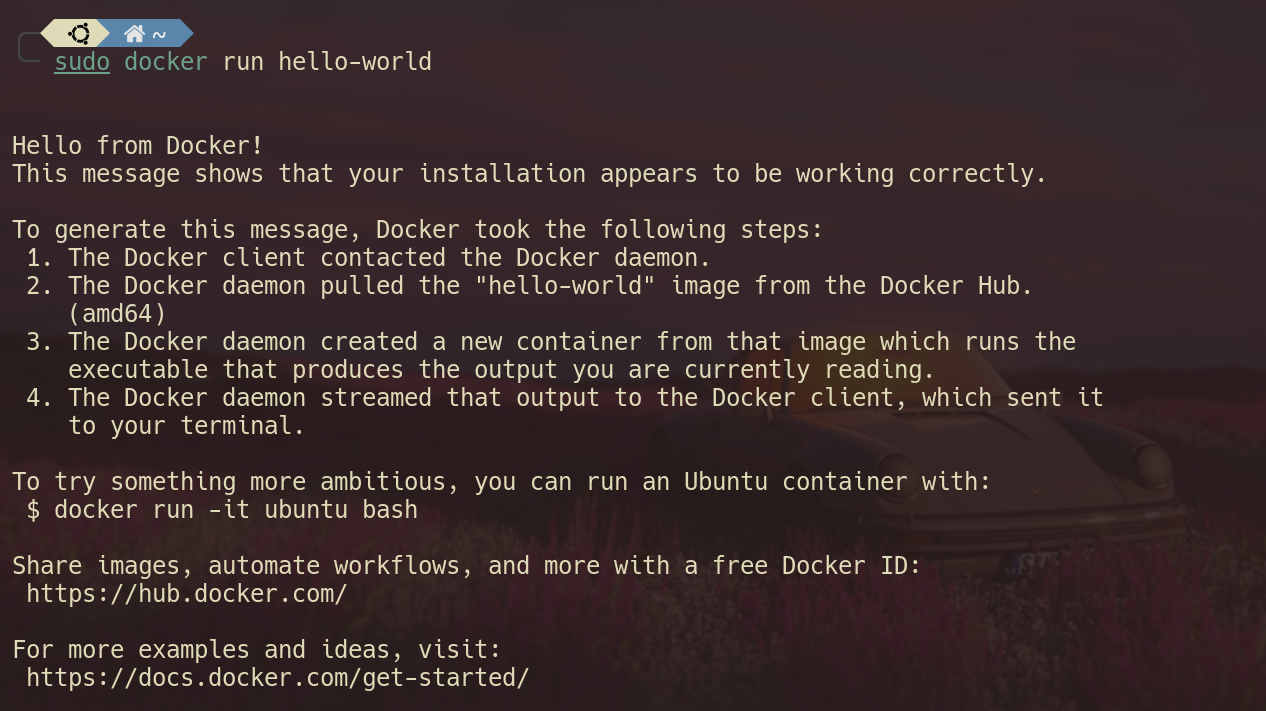
\includegraphics[width=0.6\textwidth]{images/Bloque2/hello-world.png}
    \caption{Contenedor Hello World}
    \label{fig:hello-world}
\end{figure}

\section{BenchMarks}

\subsection{¿Qué es un Benchmark?}

Un \textit{benchmark} es una prueba diseñada para medir el rendimiento de un sistema, componente o servicio informático. Estas pruebas pueden evaluar diversos aspectos, como velocidad, eficiencia, capacidad de respuesta o consumo de recursos. Existen múltiples tipos de \textit{benchmarks}, cada uno enfocado en un área específica del sistema.

Por ejemplo, para evaluar el rendimiento de un servidor DNS (que traduce nombres de dominio a direcciones IP), se pueden utilizar herramientas como \texttt{NameBench} o \texttt{GRC’s DNS Benchmark}, las cuales están diseñadas con pruebas estándar para este tipo de servicio.

\subsection{¿Por qué crear un Benchmark propio?}

Aunque existen herramientas predefinidas para realizar \textit{benchmarks}, en ocasiones es necesario programar uno propio para analizar parámetros específicos que no estén cubiertos por las herramientas existentes. Para ello, es importante considerar los siguientes elementos:

\begin{itemize}
    \item \textbf{Objetivo del Benchmark:} Definir claramente qué se desea medir, como latencia, \textit{throughput}, uso de CPU, etc.
    \item \textbf{Métricas:} Establecer las medidas que se utilizarán para evaluar el rendimiento. Esto incluye:
    \begin{itemize}
        \item Las unidades de medida (por ejemplo, milisegundos, MB/s).
        \item Las variables a observar (por ejemplo, tiempo de respuesta, carga del sistema).
        \item El método para calcular los resultados finales.
    \end{itemize}
    \item \textbf{Instrucciones de uso:} Especificar cómo ejecutar el \textit{benchmark}, el entorno requerido y los parámetros necesarios.
    \item \textbf{Ejemplo de uso y análisis de resultados:} Incluir una prueba real, interpretar los datos obtenidos y extraer conclusiones relevantes.
\end{itemize}

\subsection{OpenBenchmarking y Phoronix Test Suite (PTS)}

\subsubsection{OpenBenchmarking}

\textit{OpenBenchmarking} es un repositorio de \textit{benchmarks} de código abierto que permite a los usuarios utilizar, modificar o crear nuevas pruebas basadas en las existentes. Es una excelente fuente de inspiración para desarrollar \textit{benchmarks} personalizados.

\subsubsection{Phoronix Test Suite (PTS)}

\textit{Phoronix Test Suite (PTS)} es una plataforma asociada a \textit{OpenBenchmarking} que facilita la ejecución de \textit{benchmarks}. Es una herramienta versátil y popular para realizar pruebas de rendimiento en sistemas Linux, Windows o incluso en máquinas virtuales (MVs). Entre sus características destacan:

\begin{itemize}
    \item Amplia variedad de pruebas disponibles que se pueden ejecutar directamente desde su entorno.
    \item Integración con \textit{OpenBenchmarking}, lo que permite comparar resultados con otras máquinas.
    \item Compatibilidad con múltiples entornos, incluyendo contenedores Docker.
\end{itemize}

\subsubsection{Instalación de Phoronix Test Suite (PTS)}

La instalación de \textit{PTS} varía según el entorno utilizado:

\begin{itemize}
    \item En sistemas Debian/Ubuntu, se pueden usar paquetes precompilados.
    \item En máquinas virtuales con Rocky Linux, se recomienda el instalador universal para Linux.
    \item En Windows, también se ofrece soporte de instalación.
    \item Para las prácticas, la opción más recomendada es utilizar contenedores Docker.
\end{itemize}

\subsubsection{Enlaces útiles}

A continuación, se presentan enlaces relevantes para explorar más sobre \textit{benchmarks} y herramientas asociadas:

\begin{itemize}
    \item Software relacionado con \textit{benchmarks} en Linux: \\
    \href{https://sourceforge.net/directory/linux/?q=benchmark}{sourceforge.net/directory/linux/?q=benchmark}
    \item Repositorio de OpenBenchmarking: \href{https://openbenchmarking.org/}{openbenchmarking.org}
    \item Sitio web de Phoronix Test Suite: \href{https://www.phoronix-test-suite.com/}{phoronix-test-suite.com}
    \item Página de descargas de PTS: \href{https://www.phoronix-test-suite.com/?k=downloads}{phoronix-test-suite.com/?k=downloads}
    \item Imagen Docker recomendada para las prácticas: \href{https://hub.docker.com/r/phoronix/pts/}{hub.docker.com/r/phoronix/pts/}
\end{itemize}

\subsection{Ejercicio Opcional. Ejecutar un Benchmark}

El alumno/a debe ser capaz de utilizar \textit{Phoronix Test Suite} para:

\begin{itemize}
    \item Descargar, instalar y ejecutar un \textit{benchmark} de su elección.
    \item Almacenar y recuperar los resultados de múltiples ejecuciones del \textit{benchmark}.
    \item Explicar el objetivo del \textit{benchmark} y de los resultados obtenidos.
\end{itemize}

\subsubsection*{Solución con un benchmark distinto}

En mi caso en el propio enlace que nos ofrece la guía\footnote{\url{https://sourceforge.net/directory/linux/?q=benchmark}} he optado por instalar el que benchmarck que tiene como nombre benchmark\footnote{\url{https://sourceforge.net/projects/benchmark.mirror/}} y estoy siguiendo los pasos que aparecen en el fichero \textit{Readme.md}\footnote{Lo estoy instalando en mi máquina anfitrión.}.

Los pasos que he seguido se puede ver en la figura \ref{fig:benchmark}.

\begin{figure}[H]
    \centering
    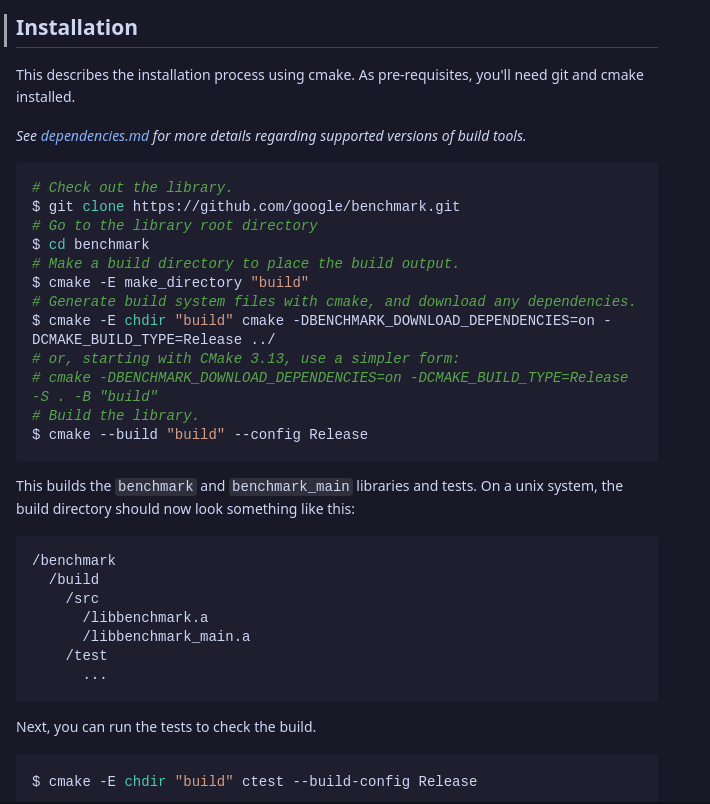
\includegraphics[width=0.6\textwidth]{images/Bloque2/installationBench.png}
    \caption{Instalación de benchmark}
    \label{fig:benchmark}
\end{figure}

Y el resultado del comando de ejecución de los tests lo puede ver en la figura \ref{fig:benchmarkResult}.

\begin{figure}[H]
    \centering
    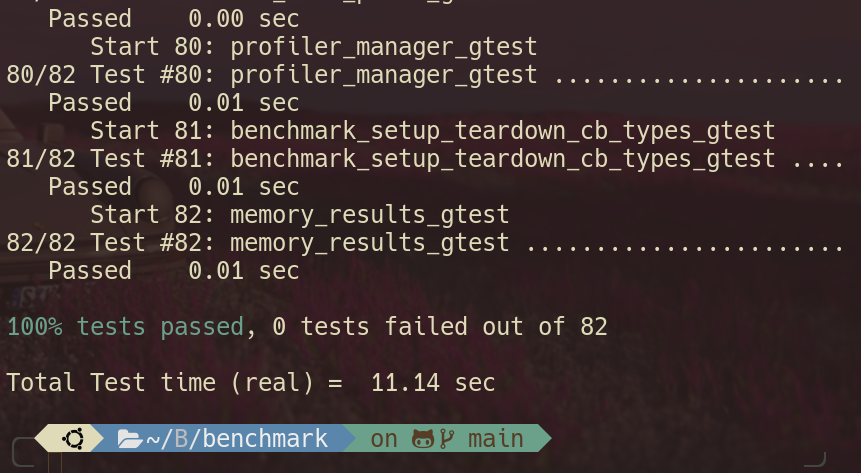
\includegraphics[width=0.6\textwidth]{images/Bloque2/resultsBench.png}
    \caption{Resultado de la ejecución del benchmark}
    \label{fig:benchmarkResult}
\end{figure}

A continuación, instalamos las librerias globales y probamos con el fichero básico que nos proporcioan, compilando y demás, nos da la salida que podemos ver en la figura \ref{fig:benchmarkResult2}.

\begin{figure}[H]
    \centering
    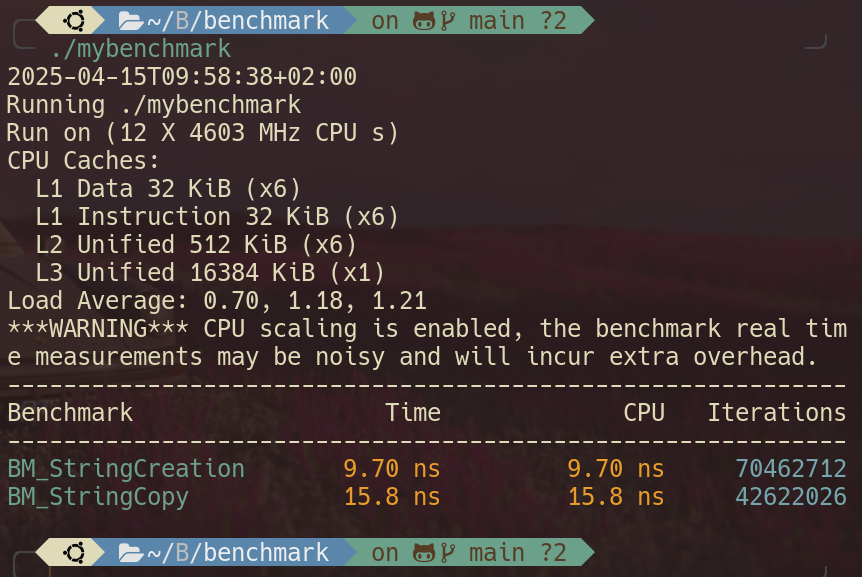
\includegraphics[width=0.6\textwidth]{images/Bloque2/resultsMYBENCHMARK.png}
    \caption{Resultado de la ejecución del benchmark}
    \label{fig:benchmarkResult2}
\end{figure}

\subsection*{Solución usando el benchmark que se especifica}

Para ello me he descargado el zip de la web y como estoy en Linux he ejecutado el comando \micode{sudo ./install.sh} y me ha instalado el programa en la ruta \micode{/usr/bin/phoronix-test-suite}.
\begin{figure}[H]
    \centering
    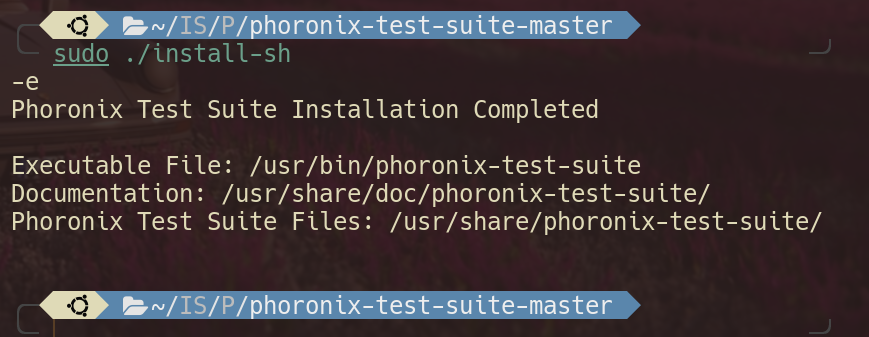
\includegraphics[width=0.6\textwidth]{images/Bloque2/installPhoro.png}
    \caption{Instalación de Phoronix Test Suite}
    \label{fig:PTS}
\end{figure}

Debemos de leer el Readme para una prueba.

En base a \textit{``phoronix-test-suite benchmark smallpt to run a simple CPU test
profile''} introducimos el comando para un primer testeo. 

% \includepdf[nup=2x2, pages=1-3, frame=true]{"../../Ficheros_Ejercicios/Ejercicios_Bloque2/resultsfirststatement.pdf"}

Donde el resultado que nos da:

\begin{lstlisting}
    resultsFirstAttempt
results


results: 

	Processor: AMD Ryzen 5 7535HS @ 4.60GHz (6 Cores / 12 Threads), Motherboard: ASUS TUF Gaming A15 FA506NC_FA506NC FA506NC v1.0 (FA506NC.308 BIOS), Chipset: AMD 17h-19h PCIe Root Complex, Memory: 2 x 8GB DDR5-4800MT/s Samsung M425R1GB4PB0-CWMOL, Disk: 512GB SAMSUNG MZVL8512HELU-00BTW + 1000GB KINGSTON SNV3S1000G, Graphics: ASUS NVIDIA GeForce RTX 3050 Mobile, Audio: NVIDIA Device 2291, Network: Realtek RTL8111/8168/8211/8411 + Realtek RTL8852BE PCIe 802.11ax

	OS: Ubuntu 24.04, Kernel: 6.11.0-21-generic (x86_64), Display Server: X Server, Compiler: GCC 13.3.0, File-System: ext4, Screen Resolution: 1920x1080


Smallpt 1.0
Global Illumination Renderer; 128 Samples
Seconds < Lower Is Better
results . 15.48 |==============================================================

\end{lstlisting}

% Otro de los benchmarks que podemos ejecutar es ``unigine-heaven''. Para ello debemos de ejecutar los comandos \micode{./phoronix-test-suite install unigine-heaven; ./phoronix-test-suite run unigine-heaven}


\subsection{Resumen: Phoronix Test Suite en Máquina Local vs Docker}

El \textit{Phoronix Test Suite} puede presentar problemas de rendimiento o fallos en una máquina local debido a dependencias faltantes, configuraciones incorrectas o conflictos en el entorno del sistema operativo. En contraste, al ejecutarlo en un contenedor Docker, se utiliza un entorno limpio y preconfigurado, optimizado por los desarrolladores para funcionar de manera eficiente.

\subsubsection{Comparativa entre Máquina Local y Docker}

\begin{table}[h!]
\centering
\begin{tabular}{|p{4cm}|p{5cm}|p{5cm}|}
\hline
\textbf{Aspecto} & \textbf{Máquina Local} & \textbf{Contenedor Docker} \\ \hline
PHP y extensiones & Puede faltar GD, bzip2, sqlite3, etc. & Todo preinstalado y configurado \\ \hline
Permisos y acceso a GPU & Problemas con \texttt{/dev/dri} u otros permisos & Aislado, puede no usar GPU directamente \\ \hline
Entorno gráfico & Falta de X11 puede romper tests gráficos & Usa \textit{fallback} o modo \textit{headless} \\ \hline
Dependencias del sistema & Conflictos o paquetes rotos & Imagen oficial limpia y probada \\ \hline
Compatibilidad de librerías & Incompatibilidades posibles & Versiones probadas y compatibles \\ \hline
\end{tabular}
\caption{Comparativa entre ejecución local y en Docker}
\end{table}

\subsubsection{Caso Específico: Benchmark \texttt{smallpt}}

El \texttt{smallpt} es un \textit{benchmark} dependiente de la CPU. Problemas como \textit{throttling}, gestión térmica deficiente o extensiones PHP faltantes pueden ralentizar su ejecución en una máquina local. En Docker, estos problemas se mitigan gracias al entorno controlado.

\subsubsection{Ventajas de Docker}

\begin{itemize}
    \item Entorno aislado y preconfigurado.
    \item Independencia de configuraciones locales.
    \item Fácil reinicio y limpieza del entorno.
    \item Uso de versiones probadas por los desarrolladores.
\end{itemize}

En resumen, ejecutar \textit{Phoronix Test Suite} en Docker garantiza mayor estabilidad y rendimiento, eliminando problemas derivados del entorno local.



Realizando diversas pruevas vemos que el comando tarda demasiado y con htop vemos que no se queda colgado pero tarda demasiado tiempo, por ende, he decidido ejecutarlo en contenedores que es como se recomienda en prácticas. 


Para ello ejecutamos los siguientes comandos:

\begin{enumerate}
    \item \micode{docker pull phoronix/pts}: para descargar la imagen de Phoronix Test Suite\footnote{El comando es de la \url{https://www.phoronix-test-suite.com/?k=downloads}.}.
    \item \micode{docker run -it --rm phoronix/pts}: para ejecutar el contenedor interactivo.
    \item \micode{phoronix-test-suite benchmark smallpt}: para ejecutar el benchmark.
\end{enumerate}

De manera que una vez que estamos dentro de la shell interactiva del docker podemos ejecutar los comandos del docker.

Los pasos a seguir para los tests son (dentro del docker de phoronix con la shell interactiva):
\begin{enumerate}
    \item Listamos los disponibles usando el comando \micode{list-avilable-test}
    \item install <test>
    \item run <test>
\end{enumerate}

En mi caso con he instalado el test \micode{php}. El resultado podemos verlo en la terminal (Ver figura \ref{fig:dockerPhoronix}). Además tenemos la opción de subirlo y poder consultarlo de manera online, en mi caso es \url{https://openbenchmarking.org/result/2504152-NE-RESULTSPH66}.

\begin{figure}[H]
    \centering
    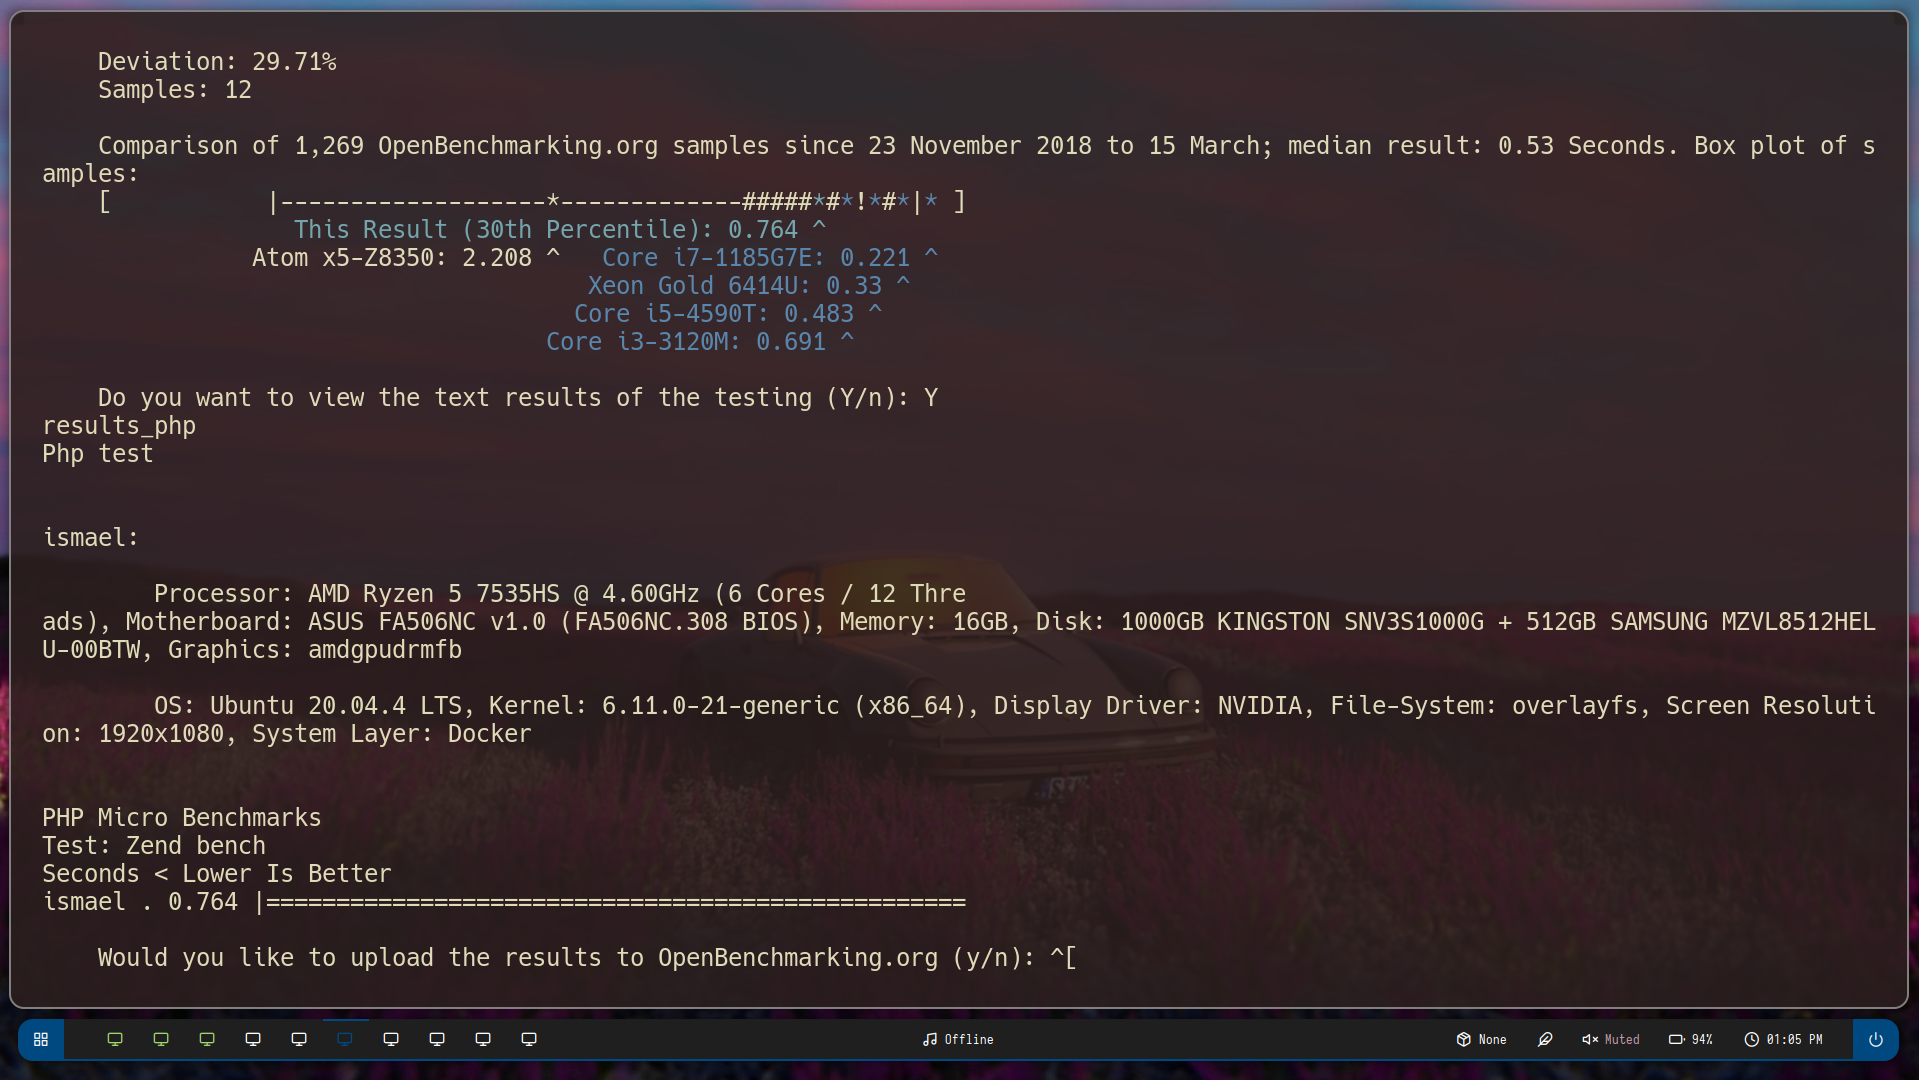
\includegraphics[width=1\textwidth]{images/Bloque2/dockerPhoronix.png}
    \caption{Resultado de la ejecución del benchmark en Docker}
    \label{fig:dockerPhoronix}
\end{figure}

\subsection*{Objetivo del Benchmark y Resultados Obtenidos}

El objetivo del benchmark realizado con \textbf{Phoronix Test Suite} fue evaluar el rendimiento del sistema, específicamente en la ejecución de pruebas micro de \textbf{PHP Zend}, bajo condiciones estándar. Este tipo de pruebas mide la eficiencia y tiempos de ejecución de componentes clave, como el procesador y la memoria, proporcionando una comparación con otros sistemas.

\subsubsection{Resultados Obtenidos}

\begin{itemize}
    \item \textbf{Tiempo promedio de ejecución}: 0.764 segundos.
    \item \textbf{Desviación estándar}: SE +/- 0.066, lo que indica una alta consistencia en los resultados.
    \item \textbf{Percentil alcanzado}: No especificado, pero los resultados muestran un rendimiento competitivo en comparación con sistemas similares.
\end{itemize}

\subsubsection{Interpretación de los Resultados}

El sistema probado, con un procesador AMD Ryzen 5 7535HS, mostró un rendimiento destacado en las pruebas de PHP Zend, con tiempos de ejecución significativamente bajos. Esto lo posiciona como una opción eficiente para entornos que requieren alta velocidad y confiabilidad en la ejecución de aplicaciones web o API basadas en PHP.

\subsubsection{Conclusión}

El benchmark confirma que el sistema es altamente eficiente en tareas relacionadas con PHP, siendo una opción ideal para desarrolladores y administradores de sistemas que buscan optimizar el rendimiento de sus servidores o aplicaciones en entornos de producción.


\subsection{Ejercicio Opcional. Comparar benchmark en contenedor y en VM}

El alumno/a ejecutará el mismo benchmark sobre: su ordenador personal, Docker en su ordenador personal y máquina virtual. Comente y justifique las posibles diferencias en los resultados obtenidos.

\subsubsection{Solución}

\begin{itemize}
    \item En cuanto a ejecutarlo en el Docker de nuestro ordenador personal, el resultado es el que hemos visto en el anterior ejercicio. Podemos ver la figura \ref{fig:dockerPhoronix}.
    \item En cuanto a la parte de ejecutarlo en nuestra máquina, vemos que anteriormente lo habíamos hecho pero tras el intento de mejorar el rendimiento instalando los drivers recomendados para ubuntu de nvidia no funcionaba, por lo que \textcolor{red}{debemos de destacar que se deben de usar los drivers de nouveau (código abierto)}, ya que si no en caso contrario se daban problemas de priorización de programas, kernel, se cuelga la detección del hardware y demás. Generando el comando básico nos quedan los resultados de nuestra máquina en la web: \url{https://openbenchmarking.org/result/2504153-NE-RESULTS0676}. De esta manera ejecutamos los comandos: 
    \begin{enumerate}
        \item \micode{phoronix-test-suite install pts/git}
        \item \micode{phoronix-test-suite run pts/git}
    \end{enumerate}

    \begin{figure}[H]
        \centering
        \begin{minipage}{0.45\textwidth}
            \centering
            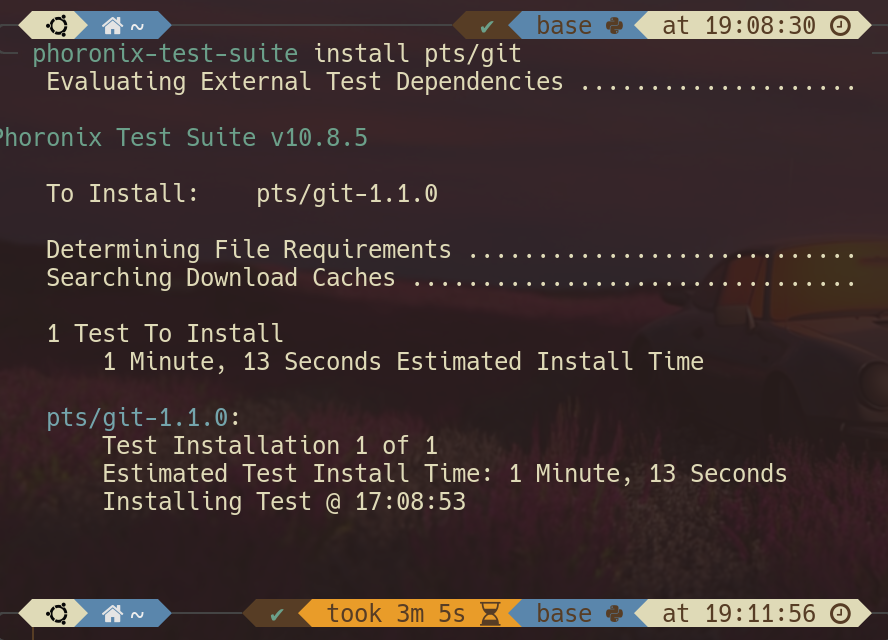
\includegraphics[width=\textwidth]{images/Bloque2/personal-phoronix-1.png}
            \caption{Instalación del test git}
            \label{fig:image1}
        \end{minipage}
        \hfill
        \begin{minipage}{0.45\textwidth}
            \centering
            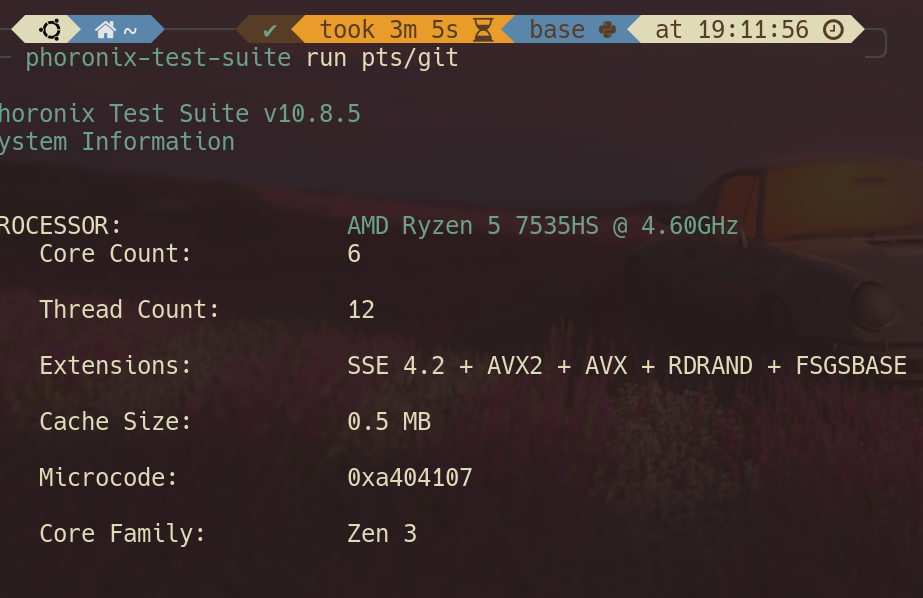
\includegraphics[width=\textwidth]{images/Bloque2/personal-phoronix-2.png}
            \caption{Run del test}
            \label{fig:image2}
        \end{minipage}
    \end{figure}
    \begin{figure}[H]
        \centering
        \begin{minipage}{0.45\textwidth}
            \centering
            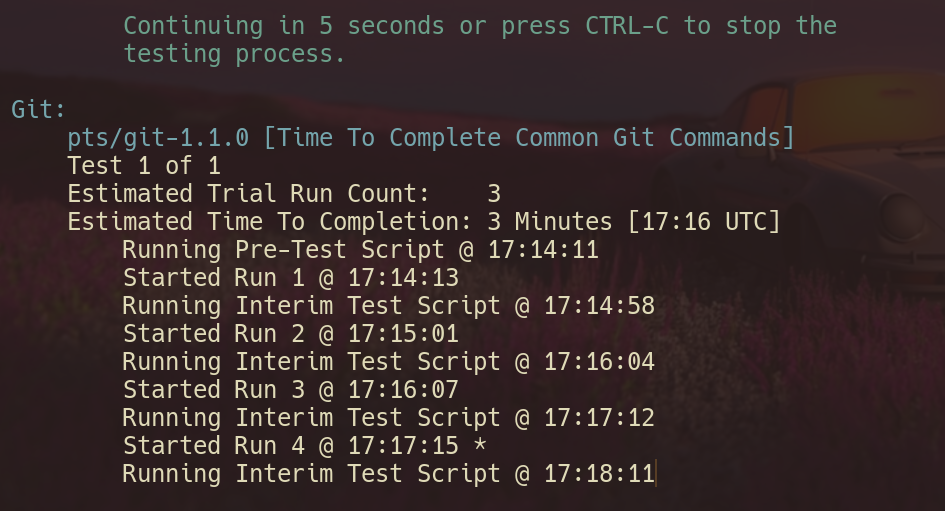
\includegraphics[width=\textwidth]{images/Bloque2/per-pho-3.png}
            \caption{Run del test en ejecución}
            \label{fig:image5}
        \end{minipage}
        \hfill
        \begin{minipage}{0.45\textwidth}
            \centering
            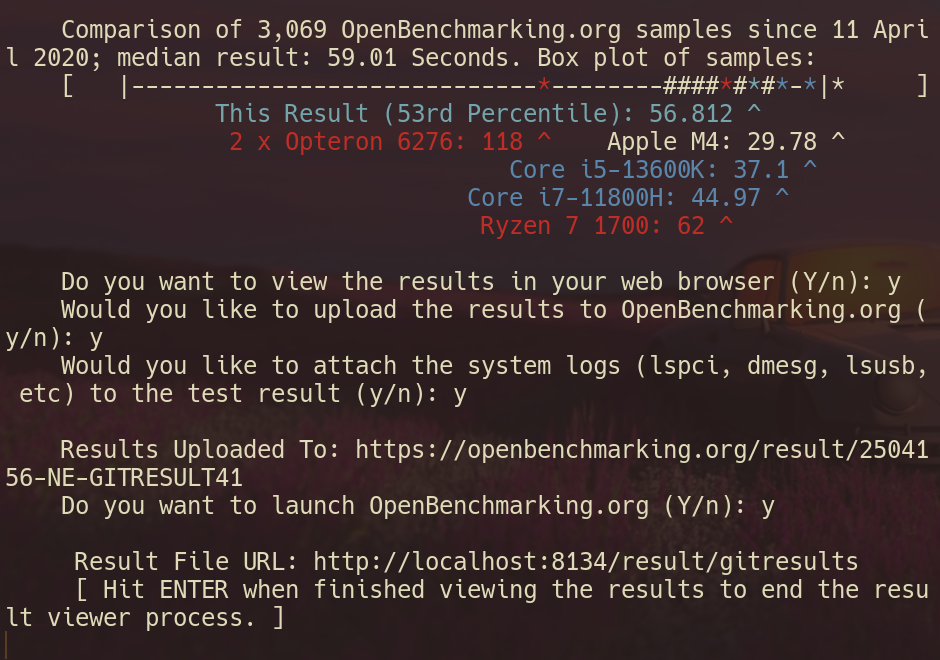
\includegraphics[width=\textwidth]{images/Bloque2/fin-git-pho.png}
            \caption{Run del test}
            \label{fig:image6}
        \end{minipage}
    \end{figure}
    Para acceder a los resultados podemos acceder al enlace: \url{https://openbenchmarking.org/result/2504156-NE-GITRESULT41}.
    \item En el caso de la máquina virtual, en mi caso he clonado la última y he cambiado de nuevo la ip. Para la descarga de phoronix podemos usar curl, wget pero yo he usado scp desde mi máquina local: \micode{scp -r Descargas/phoronix-test-suite-master ismMV01@192.168.56.106:~} (Debemos pasarlo unzipeado debido a que no tenemos la herramienta unzip).
    \begin{figure}[H]
        \centering
        \begin{minipage}{0.45\textwidth}
            \centering
            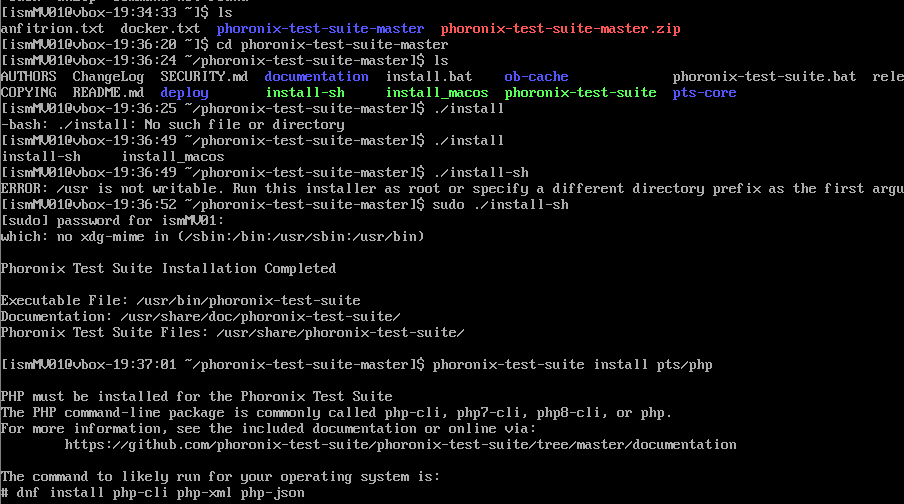
\includegraphics[width=\textwidth]{images/Bloque2/mv-pho-1.png}
            \caption{Instalaciónd de phoronix en MV Rocky, a continuación instalamos lo que nos dice, ya que instalamos pts/php}
            \label{fig:image7}
        \end{minipage}
        \hfill
        \begin{minipage}{0.45\textwidth}
            \centering
            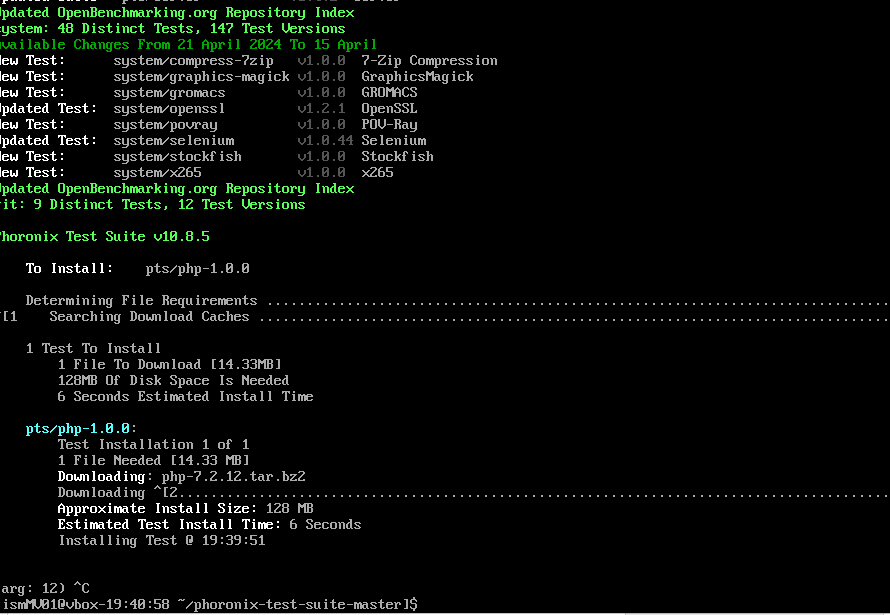
\includegraphics[width=\textwidth]{images/Bloque2/mv-pho-2.png}
            \caption{Install de pts/php}
            \label{fig:image8}
        \end{minipage}
    \end{figure}
    \begin{figure}[H]
        \centering
        \begin{minipage}{0.45\textwidth}
            \centering
            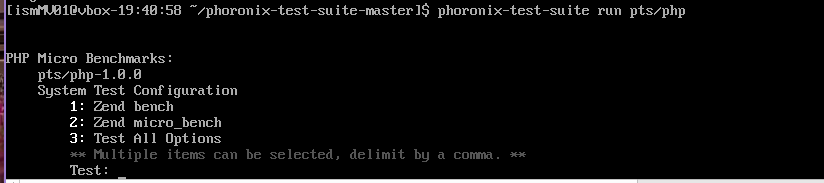
\includegraphics[width=\textwidth]{images/Bloque2/mv-pho-4.png}
            \caption{Ejecutamos el test}
            \label{fig:image9}
        \end{minipage}
        \hfill
        \begin{minipage}{0.45\textwidth}
            \centering
            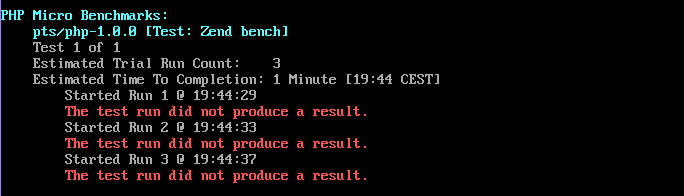
\includegraphics[width=\textwidth]{images/Bloque2/mv-pho-5.png}
            \caption{Resultado final (Vemos que no se generan resultados)}
            \label{fig:image10}
        \end{minipage}
    \end{figure}
    
\end{itemize}



\subsection{Apache Benchmarck}


\texttt{Apache Benchmark (ab)} es una herramienta de línea de comandos incluida en el servidor web Apache, diseñada para medir el rendimiento de servidores HTTP. Es especialmente útil para realizar pruebas de carga y evaluar la capacidad de respuesta de un servidor bajo diferentes niveles de tráfico.

\subsubsection{Instalación}

En la mayoría de las distribuciones Linux, \texttt{ab} se incluye como parte del paquete \texttt{apache2-utils}. Para instalarlo, ejecute:

\begin{lstlisting}[style=customstyle]
sudo apt install apache2-utils -y
\end{lstlisting}

\subsubsection{Uso Básico}

El comando básico para ejecutar \texttt{ab} es:

\begin{lstlisting}[style=customstyle]
ab -n <número_de_peticiones> -c <concurrencia> <URL>
\end{lstlisting}

\begin{itemize}
    \item \texttt{-n}: Número total de peticiones a realizar.
    \item \texttt{-c}: Número de peticiones concurrentes.
    \item \texttt{<URL>}: \\
    Dirección completa del recurso a probar (por ejemplo, \texttt{http://localhost/index.html}).
\end{itemize}

\subsubsection{Ejemplo de Uso}

Para realizar 100 peticiones con una concurrencia de 10 al servidor local, ejecute:

\begin{lstlisting}[style=customstyle]
ab -n 100 -c 10 http://localhost/
\end{lstlisting}

\subsubsection{Resultados}

El comando genera un informe detallado con métricas clave, como:

\begin{itemize}
    \item \textbf{Tiempo total de prueba:} Duración total de la prueba en segundos.
    \item \textbf{Peticiones por segundo:} Número promedio de peticiones procesadas por segundo.
    \item \textbf{Tiempo de respuesta promedio:} Tiempo promedio que tarda el servidor en responder a una petición.
    \item \textbf{Transferencia por segundo:} Cantidad de datos transferidos por segundo.
\end{itemize}

\subsubsection{Consideraciones}

\begin{itemize}
    \item \texttt{ab} no soporta HTTPS de forma nativa en algunas versiones. Para pruebas HTTPS, considere herramientas alternativas como \texttt{wrk} o \texttt{siege}.
    \item Asegúrese de que el servidor pueda manejar la carga generada por \texttt{ab} para evitar resultados poco representativos.
\end{itemize}

\subsubsection{Resumen}

\texttt{Apache Benchmark} es una herramienta sencilla pero poderosa para realizar pruebas de rendimiento en servidores HTTP. Su facilidad de uso y disponibilidad la convierten en una opción ideal para desarrolladores y administradores de sistemas que buscan evaluar la capacidad de sus servidores.

\subsection{Ejercicio Opcional. Carga Http con AB}

Ejecute el benchmark sobre los servidores Http empleados en las prácticas del Bloque 1 (Apache y Nginx). Se deja a la decisión del alumno/a la definición de los parámetros del benchmark, pero se valorará que sea capaz de definir un entorno de ejecución que eleve significativamente la carga de los servidores. El alumno/a debe ser capaz de describir en detalle los resultados obtenidos así como razonar las posibles diferencias entre los servidores.


\subsubsection{Solución}

Para hacerlo más fácil he decidido hacerlo desde un contenedor de docker en mi máquina local, los pasos son:

\begin{enumerate}
    \item Creamos el directorio donde vamos a crear el fihero docker-compose.yml y donde vamos a trabajar.
    \item Editamos el fichero \micode{docker-compose.yml} y le añadimos el siguiente contenido:
    \begin{lstlisting}[style=customstyle]
    version: '3'  # Versión del archivo docker-compose

    services:
        apache:  # Servicio para el servidor Apache
            image: httpd:2.4  # Imagen de Docker para Apache HTTP Server versión 2.4
            container_name: apache-server  # Nombre del contenedor para Apache
            ports:
                - "8080:80"  # Mapea el puerto 80 del contenedor al puerto 8080 del host

        nginx:  # Servicio para el servidor Nginx
            image: nginx:alpine  # Imagen de Docker para Nginx basada en Alpine Linux
            container_name: nginx-server  # Nombre del contenedor para Nginx
            ports:
                - "8081:80"  # Mapea el puerto 80 del contenedor al puerto 8081 del host

        ab:  # Servicio para Apache Benchmark (ab)
            image: jordi/ab  # Imagen de Docker que contiene Apache Benchmark
            container_name: ab-client  # Nombre del contenedor para Apache Benchmark
            entrypoint: tail -f /dev/null  # Mantiene el contenedor en ejecución para usarlo con `docker exec`
        \end{lstlisting}
        \item Guardamos el fichero y ejecutamos el siguiente comando para levantar los contenedores: \micode{docker-compose up -d}.
        \item Vemos que efectivamente están corriendo: \micode{docker ps}.
        \item Accedemos al contenedor de ab: \micode{docker exec -it ab-client sh}.
        \item Dentro de la shell interactiva ejecutamos los comandos:
        \begin{enumerate}
            \item \micode{ab -n 1000 -c 50 http://apache-server/ > apache.txt}: para ejecutar el benchmark en el servidor Apache y guardar los resultados en un archivo llamado \texttt{apache.txt}.
            \item \micode{ab -n 1000 -c 50 http://nginx-server/ > nginx.txt}: para ejecutar el benchmark en el servidor Nginx y guardar los resultados en un archivo llamado \texttt{nginx.txt}.
        \end{enumerate}
        \item Copiamos el contenido del contedor (este comando se ejecuta desde nuestra máquina local, no dentro del contenedor): \micode{docker cp ab-client:/apache.txt ./apache.txt ; 
        docker cp ab-client:/nginx.txt ./nginx.txt}
\end{enumerate}

En cuanto a interpretar los resultados, solo vamos a hacer el fichero \micode{apache.txt}: 

\subsubsection*{Análisis en profundidad de los resultados}

El objetivo principal del benchmark realizado con \textbf{ApacheBench (ab)} es medir el rendimiento del servidor HTTP Apache bajo condiciones de carga. Esto incluye evaluar:

\begin{itemize}
    \item \textbf{Capacidad de manejo de peticiones:} Cuántas solicitudes por segundo puede procesar el servidor.
    \item \textbf{Latencia:} Tiempo promedio de respuesta por petición.
    \item \textbf{Estabilidad:} Cómo se comporta el servidor con múltiples clientes concurrentes.
\end{itemize}

\paragraph{Información Básica del Servidor}

\begin{table}[H]
\centering
\begin{tabular}{|p{5cm}|p{5cm}|p{5cm}|}
\hline
\textbf{Campo} & \textbf{Valor} & \textbf{Explicación} \\ \hline
\textbf{Server Software} & Apache/2.4.63 & Versión del servidor Apache \\ \hline
\textbf{Hostname} & apache-server & Nombre del servidor bajo prueba \\ \hline
\textbf{Port} & 80 & Puerto HTTP estándar \\ \hline
\textbf{Document Path} & / & Página que se está solicitando (raíz) \\ \hline
\textbf{Document Length} & 45 bytes & Tamaño del contenido HTML que responde el servidor \\ \hline
\end{tabular}
\caption{Información básica del servidor}
\end{table}

\paragraph{Parámetros de Prueba}

\begin{table}[H]
\centering
\begin{tabular}{|p{5cm}|p{5cm}|p{5cm}|}
\hline
\textbf{Campo} & \textbf{Valor} & \textbf{Explicación} \\ \hline
\textbf{Concurrency Level} & 50 & Simulación de 50 clientes simultáneos \\ \hline
\textbf{Complete Requests} & 1000 & Total de peticiones realizadas al servidor \\ \hline
\textbf{Failed Requests} & 0 & Todas las solicitudes fueron exitosas \\ \hline
\end{tabular}
\caption{Parámetros de prueba}
\end{table}

\paragraph{Rendimiento del Servidor}

\begin{table}[H]
\centering
\begin{tabular}{|p{5cm}|p{5cm}|p{5cm}|}
\hline
\textbf{Campo} & \textbf{Valor} & \textbf{Explicación} \\ \hline
\textbf{Time taken for tests} & 0.165 s & Tiempo total de la prueba \\ \hline
\textbf{Requests per second} & 6057.60 req/s & Rendimiento: peticiones procesadas por segundo \\ \hline
\textbf{Time per request (mean)} & 8.254 ms & Tiempo promedio por petición individual \\ \hline
\textbf{Time per request (concurrent)} & 0.165 ms & Tiempo promedio por petición con concurrencia \\ \hline
\textbf{Transfer rate} & 1709.61 KB/s & Velocidad de transferencia promedio \\ \hline
\end{tabular}
\caption{Rendimiento del servidor}
\end{table}

\paragraph{Tiempos de Conexión y Procesamiento}

\begin{table}[H]
\centering
\begin{tabular}{|p{2cm}|p{2cm}|p{2cm}|p{2cm}|p{2cm}|p{2cm}|}
\hline
\textbf{Tipo} & \textbf{min} & \textbf{mean} & \textbf{sd} & \textbf{med} & \textbf{max} \\ \hline
\textbf{Connect} & 0 ms & 4 ms & ±1.2 & 3 ms & 8 ms \\ \hline
\textbf{Processing} & 1 ms & 4 ms & ±1.3 & 4 ms & 10 ms \\ \hline
\textbf{Waiting} & 0 ms & 3 ms & ±1.2 & 3 ms & 8 ms \\ \hline
\textbf{Total} & 4 ms & 8 ms & ±1.7 & 8 ms & 13 ms \\ \hline
\end{tabular}
\caption{Tiempos de conexión y procesamiento}
\end{table}

\paragraph{Distribución de Latencias}

\begin{table}[H]
\centering
\begin{tabular}{|l|l|}
\hline
\textbf{Percentil} & \textbf{Tiempo} \\ \hline
50\% (mediana) & 8 ms \\ \hline
66\% & 9 ms \\ \hline
75\% & 9 ms \\ \hline
90\% & 11 ms \\ \hline
100\% (máxima) & 13 ms \\ \hline
\end{tabular}
\caption{Distribución de latencias}
\end{table}


\begin{itemize}
    \item El servidor Apache demostró un rendimiento excelente, procesando más de \textbf{6000 peticiones por segundo} sin errores.
    \item La \textbf{latencia es baja y estable}, con tiempos de respuesta promedio de 8 ms y una variabilidad mínima.
    \item La distribución de latencias muestra que el \textbf{99\% de las peticiones} se completaron en 12 ms o menos, lo que indica un comportamiento altamente eficiente.
\end{itemize}

\section{Simulación de Carga con Jmeter}

\subsection{Comparativa de herramientas de pruebas de carga y rendimiento}

Existen diversas herramientas para realizar pruebas de carga y rendimiento, cada una con características específicas que las hacen más adecuadas para ciertos escenarios. A continuación, se presenta una comparación de las herramientas más populares:

\subsubsection{Apache JMeter}

Apache JMeter es una herramienta de código abierto desarrollada en Java por la Apache Software Foundation. Es ampliamente utilizada para pruebas de carga y rendimiento en aplicaciones web, bases de datos, servicios web, entre otros.

\textbf{Características principales:}
\begin{itemize}
    \item Soporte para múltiples protocolos: HTTP, FTP, JDBC, LDAP, JMS, entre otros.
    \item Permite ejecutar pruebas en modo gráfico o desde la línea de comandos, facilitando la integración en pipelines de CI/CD.
    \item Capacidad de distribuir la carga entre múltiples máquinas para simular un gran número de usuarios concurrentes.
    \item Integración con Selenium para pruebas funcionales.
\end{itemize}

\subsubsection{Flood.io (Tricentis Flood)}

Flood.io es una plataforma SaaS que permite ejecutar pruebas de carga distribuidas globalmente utilizando herramientas de código abierto como JMeter, Gatling y Selenium.

\textbf{Características principales:}
\begin{itemize}
    \item Ejecución de pruebas desde múltiples ubicaciones geográficas sin necesidad de configurar infraestructura adicional.
    \item Soporte para scripts escritos en Ruby JMeter y Flood Element (basado en TypeScript).
    \item Integración con servicios en la nube como AWS y Azure.
    \item Generación de informes detallados y monitoreo en tiempo real.
\end{itemize}

\subsubsection{Gatling}

Gatling es una herramienta de pruebas de carga y rendimiento escrita en Scala, Akka y Netty. Está diseñada para ser eficiente en el uso de recursos y permite simular un gran número de usuarios desde una sola máquina.

\textbf{Características principales:}
\begin{itemize}
    \item Uso de un lenguaje específico de dominio (DSL) para definir escenarios de prueba de manera legible y mantenible.
    \item Generación automática de informes HTML con métricas detalladas.
    \item Soporte para protocolos como HTTP, WebSockets, JMS, entre otros.
    \item Integración con herramientas de CI/CD y entornos de desarrollo.
\end{itemize}

\subsubsection{Locust}

Locust es una herramienta de pruebas de carga escrita en Python que permite definir escenarios de usuario utilizando scripts en este lenguaje.

\textbf{Características principales:}
\begin{itemize}
    \item Facilidad para escribir y mantener scripts de prueba gracias al uso de Python.
    \item Interfaz web para monitorear y controlar las pruebas en tiempo real.
    \item Capacidad de distribuir la carga entre múltiples máquinas o procesos.
    \item Soporte para protocolos como HTTP, gRPC, WebSockets, entre otros, mediante plugins.
\end{itemize}

\subsubsection{K6}

K6 es una herramienta de pruebas de carga de código abierto desarrollada por Grafana Labs. Está escrita en Go y utiliza JavaScript para definir los scripts de prueba.

\textbf{Características principales:}
\begin{itemize}
    \item Facilidad de uso para desarrolladores gracias al uso de JavaScript.
    \item Integración con pipelines de CI/CD para pruebas automatizadas.
    \item Soporte para diferentes tipos de pruebas: estrés, carga, duración, entre otras.
    \item Posibilidad de visualizar métricas en tiempo real utilizando Grafana.
\end{itemize}

\subsubsection{Artillery}

Artillery es una herramienta de pruebas de carga y rendimiento escrita en Node.js. Permite definir escenarios de prueba utilizando archivos YAML o scripts en JavaScript.

\textbf{Características principales:}
\begin{itemize}
    \item Facilidad para definir escenarios complejos de usuario.
    \item Soporte para pruebas de APIs y aplicaciones web en tiempo real.
    \item Integración con herramientas de CI/CD.
    \item Generación de informes detallados con métricas clave.
\end{itemize}

\subsubsection{Comparativa rápida}

\begin{table}[H]
\centering
\begin{tabular}{|p{3cm}|p{3cm}|p{3cm}|p{3cm}|p{3cm}|}
\hline
\textbf{Herramienta} & \textbf{Lenguaje de scripting} & \textbf{Interfaz gráfica} & \textbf{Distribución de carga} & \textbf{Protocolos soportados} \\ \hline
JMeter & Java & Sí & Sí & HTTP, FTP, JDBC, etc. \\ \hline
Flood.io & Ruby, TypeScript & Sí & Sí (en la nube) & HTTP, Selenium \\ \hline
Gatling & Scala, Java, JS & Parcial & Sí & HTTP, WebSockets \\ \hline
Locust & Python & Sí & Sí & HTTP, gRPC, etc. \\ \hline
K6 & JavaScript & No & Sí & HTTP, WebSockets \\ \hline
Artillery & JavaScript, YAML & No & Sí & HTTP, WebSockets \\ \hline
\end{tabular}
\caption{Comparativa de herramientas de pruebas de carga y rendimiento}
\end{table}

\subsection{Instalación de Jmeter}

\textit{Nota:} en cuanto a la instalación de Jmeter, lo haremos en nuestra máquina local.

Para la instalación debemos de clonar el repositorio \url{https://github.com/davidPalomar-ugr/iseP4JMeter.git} y acto seguido entramos y lanzamos el docker (podemos usar -d para que sea en segundo plano) con el comando: \micode{docker compose up -d}.

\subsection{Detalles sobre el Dockerfile y Docker-Compose}

El \texttt{Dockerfile} es el archivo donde se especifican todos los comandos necesarios para crear una imagen de Docker y las acciones que debe realizar sobre esta, como copiar archivos, instalar paquetes o modificar configuraciones. Desde un punto de vista abstracto, podríamos considerarlo como un \textit{playbook} que Docker aplica al levantar el contenedor.

En este caso, dos elementos clave en el \texttt{Dockerfile} son la configuración del contenedor en lo que respecta a red y almacenamiento. A continuación, se describen los \texttt{Dockerfiles} utilizados en los contenedores de la aplicación y la base de datos:

\subsubsection{Dockerfile de la aplicación (Node.js)}


\begin{lstlisting}[language=Dockerfile]
FROM node:16.13.0-stretch
RUN mkdir -p /usr/src/app
COPY . /usr/src/app
EXPOSE 3000
WORKDIR /usr/src/app
RUN ["npm", "install"]
ENV NODE_ENV=production
CMD ["npm","start"]
\end{lstlisting}

En este archivo:
\begin{itemize}
    \item Se utiliza la imagen base \texttt{node:16.13.0-stretch}, que incluye Node.js versión 16.13.0 y Debian Stretch como sistema operativo.
    \item Se crea un directorio para la aplicación y se copian los archivos del repositorio al contenedor.
    \item Se expone el puerto \texttt{3000}, que será mapeado al puerto del anfitrión.
    \item Se configura la variable de entorno \texttt{NODE\_ENV} como \texttt{production}.
    \item Finalmente, se ejecuta el comando \texttt{npm start} para iniciar la aplicación.
\end{itemize}

\subsubsection{Dockerfile de la base de datos (MongoDB)}

\begin{lstlisting}[language=Dockerfile]
FROM mongo:6
COPY ./scripts/* /tmp/
RUN chmod 755 /tmp/initializeMongoDB.sh
WORKDIR /tmp
CMD ./initializeMongoDB.sh
\end{lstlisting}

En este archivo:
\begin{itemize}
    \item Se utiliza la imagen base \texttt{mongo:6}.
    \item Se copian los scripts necesarios al contenedor y se ajustan los permisos.
    \item Se establece el directorio de trabajo en \texttt{/tmp}.
    \item Finalmente, se ejecuta un script para inicializar y rellenar la base de datos.
\end{itemize}

\subsubsection{Archivo \texttt{docker-compose.yml}}

La herramienta \texttt{docker-compose} permite configurar varios contenedores para que trabajen juntos como un único servicio. El archivo \texttt{docker-compose.yml} especifica los siguientes elementos:



\begin{lstlisting}[language=yaml]
version: '2.0'
services:
  # MongoDB based in the original Mongo Image
  mongodb:
    image: mongo:6
    ports:
      - "27017:27017"
  # Initialize mongodb with data
  mongodbinit:
    build: ./mongodb
    links:
      - mongodb
  # Nodejs App
  nodejs:
    build: ./nodejs
    ports:
      - "3000:3000"
    links:
      - mongodb
\end{lstlisting}

En este archivo:
\begin{itemize}
    \item Se define un servicio para MongoDB, exponiendo el puerto \texttt{27017}.
    \item Se configura un servicio para inicializar MongoDB con datos, que depende del contenedor \texttt{mongodb}.
    \item Se define un servicio para la aplicación Node.js, exponiendo el puerto \texttt{3000} y enlazándolo con el contenedor \texttt{mongodb}.
\end{itemize}

\begin{figure}[H]
    \centering
    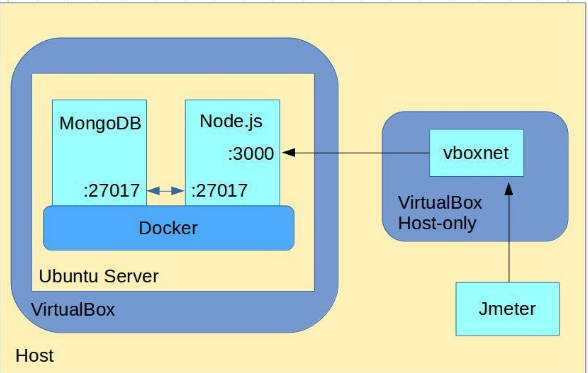
\includegraphics[width=0.6\textwidth]{images/Bloque2/abs-jmeter.png}
    \caption{Descripción de los niveles de abstracción y los distintos elementos en ejecución.}
    \label{fig:docker-compose}
\end{figure}

Esta configuración permite que los contenedores trabajen en conjunto, utilizando la red \texttt{bridge} de Docker para comunicarse entre ellos. Para más detalles, consulte la documentación oficial de Docker y Docker Compose.

\subsection{Ejercicio Obligatorio. Simulación de Carga Http con JMeter}

El repositorio \url{https://github.com/davidPalomar-ugr/iseP4JMeter.git} contiene la aplicación objeto de la prueba de carga y una descripción de los requerimientos sobre la carga a simular. Siga las instrucciones y elabore la prueba de carga con JMeter.

El alumno/a deberá realizar todo el ejercicio en un directorio que contendrá todos los artefactos necesarios para la ejecución de la prueba de carga con JMeter. Dentro de la prueba de carga, los paths a los archivos se definirán de forma relativa para que la ejecución sea independiente de la localización del directorio. Como validación final, el alumno/a debe ser capaz de ejecutar la prueba de carga por línea de comandos (sin interfaz gráfica) desde cualquier directorio de su equipo.

\subsubsection*{Solución}

Para ejecutarlo mediante la línea de comandos sin interfaz gráfica:
\begin{lstlisting}[style=customstyle]
    ./jmeter -n -t /ruta/completa/a/tu/archivo.jmx -l /ruta/completa/a/tu/archivo_resultados.jtl
\end{lstlisting}

\begin{enumerate}
    \item Primero he instalado lo que se conoce como Apache Jmeter, que es una herramienta de pruebas de carga y rendimiento. Para ello he usado el siguiente comando:
    \begin{enumerate}
        \item \micode{wget https://dlcdn.apache.org//jmeter/binaries/apache-jmeter-5.6.3.tgz}
        \item \micode{tar -xvzf apache-jmeter-5.6.3.tgz}
        \item \micode{mv apache-jmeter-5.6.3 ~/jmeter}
    \end{enumerate}
    Y para ejecutarlo:
    \begin{itemize}
        \item Interfaz gráfica: \micode{cd ~/jmeter/bin ; ./jmeter}
        \item Para la línea de comandos: \micode{./jmeter -n -t ruta/al/archivo.jmx -l resultados.jtl -j log.log}
    \end{itemize}
    Para poder lanzar \textit{Jmeter} desde cualquier directorio vamos a añadirlo al path:
    \begin{enumerate}
        \item Abre tu archivo de configuración del shell (por ejemplo \texttt{~/.bashrc} o \texttt{~/.zshrc}):
        \begin{lstlisting}[style=customstyle]
    nano ~/.bashrc
        \end{lstlisting}
        \item Agrega al final:
        \begin{lstlisting}[style=customstyle]
    export PATH="$PATH:$HOME/jmeter/bin"
        \end{lstlisting}
        \item Aplica los cambios:
        \begin{lstlisting}[style=customstyle]
    source ~/.bashrc
        \end{lstlisting}
    \end{enumerate}

    Ahora puedes lanzar \texttt{jmeter} desde cualquier directorio.

    \item Tras clonar el respositorio y demás, creamos un directorio para entregar, para ello ejecutamos el comando: \texttt{mkdir -p jmeter\_test/\{scripts,data,results,logs\}}  
    \item A continuación debemos de ir añadiendo lo necesario para crear el fichero \texttt{.jmx} que queda de la siguiente manera:
    \begin{enumerate}
            \item \textbf{Parametrización de HOST y PUERTO.} \\
            Definimos las variables \texttt{HOST} y \texttt{PORT} para facilitar la configuración del test. Esto se realiza en el Plan de Pruebas: \texttt{Editar $\rightarrow$ Añadir $\rightarrow$ Configuración $\rightarrow$ Variables de Usuario}.

            \item \textbf{Creación del grupo de hebras para los alumnos.} \\
            Creamos un grupo de hebras con 3 usuarios para simular las peticiones de los alumnos. Para ello, en el Plan de Pruebas: \texttt{Editar $\rightarrow$ Añadir $\rightarrow$ Hilos (Usuarios) $\rightarrow$ Grupo de Hilos}.

            \item \textbf{Añadir la petición de acceso al servidor.} \\
            Configuramos los valores por defecto para las peticiones HTTP, haciendo referencia a las variables \texttt{HOST} y \texttt{PORT}. En el Plan de Pruebas: \texttt{Editar $\rightarrow$ Añadir $\rightarrow$ Configuración $\rightarrow$ Valores por Defecto para Petición HTTP}.

            \item \textbf{Definir la autorización básica a la API.} \\
            Configuramos la autorización básica con los datos proporcionados: \texttt{URL Base: http://\$\{HOST\}:\$\{PORT\}/api/v1/auth/login}, \texttt{Usuario: etsiiApi}, \texttt{Contraseña: laApiDeLaETSIIDaLache}. En el Plan de Pruebas: \texttt{Editar $\rightarrow$ Añadir $\rightarrow$ Configuración $\rightarrow$ Gestor de Autorización HTTP}.

            \item \textbf{Definir las credenciales para los alumnos.} \\
            Indicamos que las credenciales de los alumnos se encuentran en el archivo \texttt{alumnos.csv}, cuyos campos son \texttt{usuario} y \texttt{contraseña}. En el grupo \texttt{Alumnos}: \texttt{Editar $\rightarrow$ Añadir $\rightarrow$ Configuración $\rightarrow$ Configuración del CSV Data Set}.

            \item \textbf{Crear una petición POST para los alumnos.} \\
            Añadimos una petición HTTP para realizar el login de los alumnos. En el grupo \texttt{Alumnos}: \texttt{Editar $\rightarrow$ Añadir $\rightarrow$ Muestreador $\rightarrow$ Petición HTTP}.

            \item \textbf{Recuperar el token de autenticación.} \\
            Configuramos un extractor de expresiones regulares para capturar el token devuelto por el servidor tras una autenticación válida. En \texttt{Login Alumnos}: \texttt{Editar $\rightarrow$ Añadir $\rightarrow$ Post Procesadores $\rightarrow$ Extractor de Expresiones Regulares}.

            \item \textbf{Añadir un temporizador aleatorio.} \\
            Para simular accesos más realistas, añadimos un temporizador que siga una distribución Gaussiana. En el grupo \texttt{Alumnos}: \texttt{Editar $\rightarrow$ Añadir $\rightarrow$ Temporizador $\rightarrow$ Temporizador Aleatorio Gaussiano}.

            \item \textbf{Recuperar los datos de los alumnos.} \\
            Creamos una petición GET para obtener los datos de los alumnos. En el grupo \texttt{Alumnos}: \texttt{Editar $\rightarrow$ Añadir $\rightarrow$ Muestreador $\rightarrow$ Petición HTTP}.

            \item \textbf{Resolver problemas de token inválido.} \\
            Configuramos un gestor de cabecera HTTP para manejar problemas relacionados con la validez del token. En el grupo \texttt{Alumnos}: \texttt{Editar $\rightarrow$ Añadir $\rightarrow$ Configuración $\rightarrow$ Gestor de Cabecera HTTP}.

            \item \textbf{Crear el grupo de hebras para los administradores.} \\
            Creamos un grupo de hebras con 2 usuarios para simular las peticiones de los administradores. En el Plan de Pruebas: \texttt{Editar $\rightarrow$ Añadir $\rightarrow$ Hilos (Usuarios) $\rightarrow$ Grupo de Hilos}.

            \item \textbf{Definir las credenciales para los administradores.} \\
            Indicamos que las credenciales de los administradores se encuentran en el archivo \texttt{administradores.csv}, cuyos campos son \texttt{usuario} y \texttt{contraseña}. En el grupo \texttt{Administradores}: \texttt{Editar $\rightarrow$ Añadir $\rightarrow$ Configuración $\rightarrow$ Configuración del CSV Data Set}.

            \item \textbf{Crear una petición POST para los administradores.} \\
            Añadimos una petición HTTP para realizar el login de los administradores. En el grupo \texttt{Administradores}: \texttt{Editar $\rightarrow$ Añadir $\rightarrow$ Muestreador $\rightarrow$ Petición HTTP}.

            \item \textbf{Recuperar el token de los administradores.} \\
            Configuramos un extractor de expresiones regulares para capturar el token devuelto por el servidor tras una autenticación válida. En \texttt{Login Administradores}: \texttt{Editar $\rightarrow$ Añadir $\rightarrow$ Post Procesadores $\rightarrow$ Extractor de Expresiones Regulares}.

            \item \textbf{Añadir un muestreador de acceso a log.} \\
            Configuramos un muestreador para registrar los accesos al sistema. En el grupo \texttt{Administradores}: \texttt{Editar $\rightarrow$ Añadir $\rightarrow$ Muestreador $\rightarrow$ Muestreador de Acceso a Log}.

            \item \textbf{Añadir un temporizador aleatorio.} \\
            Añadimos un temporizador que siga una distribución Gaussiana. En el grupo \texttt{Administradores}: \texttt{Editar $\rightarrow$ Añadir $\rightarrow$ Temporizador $\rightarrow$ Temporizador Aleatorio Gaussiano}.

            \item \textbf{Añadir elementos de generación de informe.} \\
            Configuramos receptores para visualizar los resultados: \texttt{Ver Árbol de Resultados}, \texttt{Reporte Resumen} e \texttt{Informe Agregado}. En el grupo \texttt{Administradores}: \texttt{Editar $\rightarrow$ Añadir $\rightarrow$ Receptor}.
    \end{enumerate}

    El fichero \texttt{.jmx} resultante se encuentra en el directorio \texttt{scripts} del repositorio.

\end{enumerate}

\section{Monitoring}

La monitorización es un componente fundamental en la operación de servicios IT y constituye la base de metodologías modernas de administración como \textit{DevOps} o \textit{Site Reliability Engineering} (SRE). Su objetivo es proporcionar visibilidad sobre el estado, rendimiento y utilización de los recursos de los sistemas informáticos, facilitando así la toma de decisiones, la detección de anomalías y la optimización continua.

\subsection{Top}

\texttt{top} es una herramienta clásica y ampliamente utilizada para obtener métricas en tiempo real sobre los procesos del sistema y el uso de los recursos computacionales del servidor. Su interfaz de texto, compatible con entornos sin interfaz gráfica, junto con su disponibilidad en prácticamente todas las plataformas Unix-like, la convierten en una utilidad esencial para administradores de sistemas.

\texttt{htop} es una versión mejorada de \texttt{top} que ofrece capacidades de visualización extendidas, como una interfaz interactiva más amigable, posibilidad de ordenar columnas dinámicamente, y representación gráfica del uso de CPU, memoria y procesos activos.

La herramienta \texttt{top} muestra una lista de métricas que han trascendido el ámbito de Linux y que todo administrador/a debe conocer. Es fundamental familiarizarse con estos indicadores, ser capaz de explicar su significado y justificar su valor en función de la carga actual del sistema.

Internamente, \texttt{top} no genera datos nuevos, sino que recopila y presenta información que ya está disponible a través del sistema operativo. Otras herramientas como \texttt{uptime}, \texttt{free} o \texttt{vmstat} ofrecen vistas alternativas de estas mismas fuentes, devolviendo datos por \texttt{stdout}, lo que las hace útiles para su integración en scripts de automatización.

Una fuente crítica para todas estas herramientas es el sistema de archivos \texttt{/proc}, un sistema de archivos virtual que contiene información dinámica sobre el estado del sistema. Dentro de este directorio se encuentran ficheros como:

\begin{itemize}
  \item \texttt{/proc/loadavg}: carga media del sistema.
  \item \texttt{/proc/meminfo}: información sobre la memoria.
  \item \texttt{/proc/uptime}: tiempo que el sistema lleva encendido.
  \item \texttt{/proc/stat}: estadísticas globales del sistema, incluyendo CPU.
  \item \texttt{/proc/cpuinfo}: detalles del procesador.
\end{itemize}

Asimismo, el directorio \texttt{/proc/<pid>} (donde \texttt{<pid>} es el identificador de un proceso) contiene información detallada sobre cada proceso en ejecución, como su estado, consumo de memoria, uso de CPU y archivos abiertos.

En resumen, \texttt{top} y sus utilidades relacionadas permiten a los administradores comprender el comportamiento del sistema y tomar decisiones fundamentadas para su gestión y optimización.


\subsection{4.1.1.- Ejercicio Opcional. Stress + Top}

Simule una carga de trabajo en su equipo anfitrión o en un MV empleando el programa \texttt{stress}. 

Monitorice con \texttt{Top} (o \texttt{Htop}) la evolución de la carga y justifique razonadamente los valores obtenidos.

\subsubsection*{Solución}

En mi caso he decidido hacerlo en mi máquina local, pero también se puede hacer en la MV.

\begin{enumerate}
    \item Para ello antes de nada debemos de instalar el programa \texttt{stress} y los que sea necesarios en nuestra máquina local, para ello ejecutamos el siguiente comando:

    \begin{lstlisting}[style=customstyle]
    sudo apt update
    sudo apt install stress htop
    \end{lstlisting}

    \item Antes de lanzar el comando \texttt{stress}, vemos cuantos núcleos tiene mi máquina local, para ello ejecutamos el siguiente comando:
    \begin{lstlisting}[style=customstyle]
    nproc
    \end{lstlisting}

    \item Ejecutamos el comando \texttt{stress --cpu 4 --timeout 60} para generar carga en 4 núcleos durante 60 segundos.
    
    \item Como podemos ver en la la figura \ref{fig:stress-top}, el uso de CPU ha aumentado considerablemente, aproximándose al 100\% y que los recursos que consume aumentan.
    \begin{figure}[H]
        \centering
        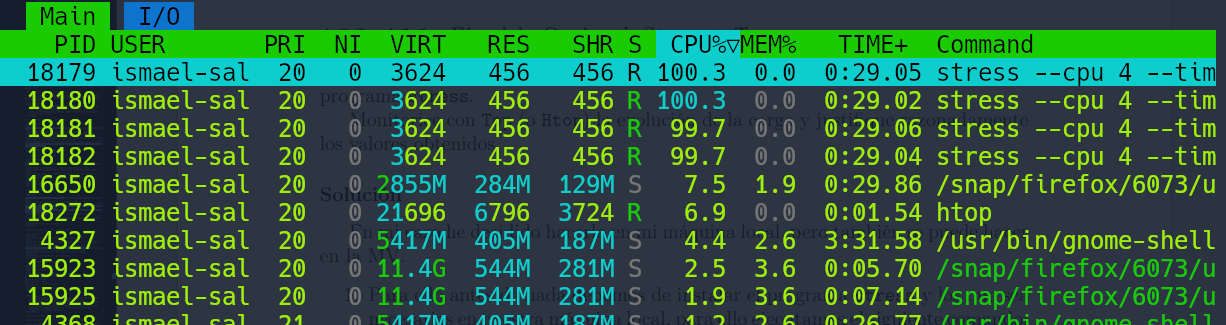
\includegraphics[width=0.6\textwidth]{images/Bloque2/htop.png}
        \caption{Ejecución del comando stress y monitorización con top}
        \label{fig:stress-top}
    \end{figure}

    \subsubsection*{Justificación razonada de los resultados}

    \paragraph{Carga del sistema (load average):}
    El valor de \textit{load average} refleja el número de procesos que están esperando utilizar la CPU. Al ejecutar el comando \texttt{stress --cpu 4}, el \textit{load average} aumentó hasta aproximadamente 4.00 en el intervalo de 1 minuto. Este valor es consistente con el número de núcleos disponibles en el sistema (4). Si el \textit{load average} hubiera superado el número de núcleos, habría indicado una sobrecarga del sistema.

    \paragraph{Uso de CPU:}
    Cada hilo generado por \texttt{stress} consumió un núcleo al 100\%. Esto se verificó mediante la herramienta \texttt{htop}, que mostró 4 procesos \texttt{stress} activos, cada uno utilizando entre el 99\% y el 100\% de la CPU. Este comportamiento confirma que los núcleos estaban completamente ocupados procesando las tareas generadas por \texttt{stress}.

    \paragraph{Uso de RAM:}
    En esta prueba no se utilizó la opción \texttt{--vm}, por lo que no se observó un uso significativo de memoria RAM. Si se hubiera incluido esta opción, la memoria libre habría disminuido proporcionalmente a la cantidad solicitada por cada hilo, lo que podría haber afectado al rendimiento general del sistema.

    \paragraph{Comportamiento general:}
    El sistema no mostró síntomas de ralentización significativa durante la prueba, lo que indica que la carga generada por \texttt{stress} fue manejada adecuadamente por los recursos disponibles. Esto demuestra que el sistema respondió de manera eficiente a las tareas intensivas generadas artificialmente, manteniendo un comportamiento estable bajo la carga simulada.



\end{enumerate}

\section{Programación de tareas periódicas con cron}

\subsection*{Tareas Periódicas en Administración de Servidores}

En la administración de servidores, es habitual automatizar tareas de mantenimiento que se repiten con cierta frecuencia. Estas tareas incluyen la verificación del estado del sistema, la rotación de archivos de registro y la limpieza de recursos. De igual forma, en procesos de monitorización, se suelen programar ejecuciones periódicas para recolectar información del sistema.

Aunque existen herramientas modernas que permiten una gestión más avanzada de estas tareas, muchas administraciones siguen utilizando herramientas tradicionales debido a su simplicidad, compatibilidad y extensa adopción en distintos entornos.

\subsection{Ejercicio Opcional. Tarea periódica con cron}

Empleando \texttt{cron} y la utilidad \texttt{logger}, programe una tarea periódica en su espacio de usuario que genere un mensaje de log con la etiqueta \texttt{ISE} y cuyo texto tenga la forma:

\begin{center}
\texttt{<SusIniciales>: <Fecha y hora actual> – <Carga actual del Sistema>}
\end{center}

\subsection*{Solución}

Es simple, tan solo debemos de:
\begin{enumerate}
    \item Crear un script con el código que se encuentra en el fichero del repositorio.
    \item Dar permisos de ejecución al script.
    \item Ejecutar el comando \texttt{crontab -e} para editar el archivo de configuración de cron.
    \item Añadir la siguiente línea al final del archivo:
    \begin{lstlisting}[style=customstyle]   
* * * * * /ruta/al/script.sh
    \end{lstlisting}
    \item Guardar y salir del editor.
    \item Verficamos usando el comando \texttt{journalctl -t ISE} que se han generado los logs.
    \item Comprobar los logs generados en el archivo de log especificado en el script.
\end{enumerate}

\section{Logs del sistema}

Una forma básica de monitorización consiste en analizar los registros (\textit{logs}) generados por el sistema operativo y los servicios instalados. En sistemas Linux, estos logs se almacenan en el directorio \texttt{/var/log}, el cual contiene tanto registros del propio sistema (como \texttt{messages}, \texttt{secure}, \texttt{lastlog}, \texttt{btmp}, entre otros) como de servicios adicionales, por ejemplo servidores web.

Muchos de estos archivos están en formato de texto plano, lo que permite su visualización mediante comandos comunes como \texttt{cat}, \texttt{grep}, \texttt{less}, \texttt{more} o \texttt{tail}. Es común encontrar múltiples versiones de un mismo log, como \texttt{cron}, \texttt{cron-20240222}, \texttt{cron-20240225}, etc. Estas versiones corresponden a rotaciones del archivo original, las cuales permiten mantener el tamaño de los logs en niveles razonables para facilitar su lectura y gestión.

La herramienta responsable de esta rotación es \texttt{logrotate}, que normalmente se ejecuta como una tarea periódica definida en \texttt{cron}. Entre sus funcionalidades se incluyen la rotación basada en tamaño o antigüedad, la compresión de logs rotados y la ejecución de acciones tras la rotación, como notificar a un servicio.

La configuración general de \texttt{logrotate} se encuentra en \texttt{/etc/logrotate.conf}, mientras que las configuraciones específicas por servicio están en \texttt{/etc/logrotate.d/}. Además, algunos servicios como Apache incluyen utilidades propias para la rotación, como \texttt{rotatelogs}, la cual permite la gestión de logs sin necesidad de reiniciar el servicio y es fácil de integrar con aplicaciones que escriben en la salida estándar.

Cabe mencionar que ciertos logs están en formato binario y requieren comandos específicos para su consulta, como \texttt{last} o \texttt{who} para los archivos \texttt{btmp} y \texttt{wtmp}.

Finalmente, el sistema \texttt{systemd} centraliza la gestión de logs mediante el servicio \texttt{systemd-journald}. Por defecto, este servicio almacena los logs de manera volátil, pero es posible habilitar su persistencia creando el directorio \texttt{/var/log/journal}. Para visualizar estos registros, se utiliza el comando \texttt{journalctl}.

\subsection{Ejercicio Opcional. Logs de arranque del sistema}

Consulte los logs del último arranque de una MV Rocky empleando \texttt{journalctl}. Concretamente, presente mensajes de niveles \texttt{warning} o más importantes.

\section*{Consulta de Logs de Arranque con \texttt{journalctl}}

El objetivo de este ejercicio es consultar los registros del sistema generados durante el último arranque de una máquina virtual Rocky Linux, utilizando la herramienta \texttt{journalctl}, y filtrar únicamente aquellos mensajes cuyo nivel de prioridad sea \texttt{warning} o superior.

\subsection*{Paso 1: Acceder al sistema}

Abra una terminal en la máquina virtual Rocky Linux, ya sea de forma local o mediante acceso remoto (por ejemplo, SSH).

\subsection*{Paso 2: Verificar el servicio \texttt{systemd-journald}}

Antes de consultar los registros, asegúrese de que el servicio de registro del sistema se encuentra en ejecución. Para ello, ejecute el siguiente comando:

\begin{verbatim}
systemctl status systemd-journald
\end{verbatim}

El resultado debe indicar que el servicio está activo y en ejecución (\texttt{active (running)}).

\subsection*{Paso 3: Consultar los logs del último arranque}

Para obtener únicamente los mensajes correspondientes al último arranque del sistema y cuyo nivel de prioridad sea \texttt{warning} o más grave, utilice el siguiente comando:

\begin{verbatim}
journalctl -b -p warning
\end{verbatim}

Este comando muestra los mensajes generados desde el último arranque con prioridad \texttt{warning}, \texttt{err}, \texttt{crit}, \texttt{alert} o \texttt{emerg}.

\subsection*{Paso 4: Visualización y exportación de los logs (opcional)}

Si desea navegar por los mensajes de manera más cómoda, puede usar un paginador como \texttt{less}:

\begin{verbatim}
journalctl -b -p warning | less
\end{verbatim}

Para guardar los registros en un archivo de texto, use la redirección de salida:

\begin{verbatim}
journalctl -b -p warning > logs_arranque.txt
\end{verbatim}

\subsection*{Paso 5: Consultar arranques anteriores (opcional)}

En caso de querer revisar los logs de un arranque anterior al actual, utilice la opción \texttt{-b -1}, como se muestra a continuación:

\begin{verbatim}
journalctl -b -1 -p warning
\end{verbatim}

\subsection*{Resultado esperado}

La salida del comando debe contener mensajes con advertencias, errores o alertas que hayan ocurrido durante el arranque del sistema, lo cual permite al administrador identificar posibles incidencias o configuraciones incorrectas.

\newpage
\section{Grafana + Prometheus}

Grafana es una herramienta de código abierto orientada a la observabilidad y monitorización de sistemas. Su arquitectura se basa en componentes como los \textit{dashboards}, los paneles y las alertas, permitiendo construir una pila de observabilidad personalizada para distintos entornos. Esta herramienta ofrece opciones tanto de despliegue autogestionado como de servicio en la nube, adaptándose así a diferentes presupuestos y necesidades organizativas.

Grafana proporciona funcionalidades avanzadas de visualización y definición de alertas sobre datos de telemetría. Sin embargo, no se encarga directamente de la recolección ni del almacenamiento de estos datos. Para ello, se emplea Prometheus, una solución específicamente diseñada para extraer, almacenar y gestionar información de monitorización de manera eficiente.

Prometheus destaca por su capacidad para manejar series temporales, su modelo de datos abierto y flexible, y por soportar métricas estandarizadas. Aunque incluye funciones básicas de visualización y gestión de alertas, estas son limitadas, por lo que suele combinarse con Grafana para conformar una solución más completa. Esta combinación es ampliamente utilizada en infraestructuras tecnológicas modernas.

Ambos servicios pueden instalarse localmente en una máquina virtual Rocky Linux o en el sistema anfitrión, siempre que sea compatible. Sin embargo, para entornos de práctica o desarrollo, se recomienda su ejecución mediante contenedores Docker utilizando \texttt{docker-compose}.

\subsection*{Despliegue con Docker Compose}

Para iniciar los servicios de Prometheus y Grafana en contenedores Docker, se requiere crear un directorio (por ejemplo, \texttt{progra}) y dentro de él, definir los siguientes archivos:

\subsubsection*{Archivo \texttt{docker-compose.yml}}

\begin{verbatim}
version: "3"
services:
  prometheus:
    image: prom/prometheus:v2.50.0
    ports:
      - 9090:9090
    volumes:
      - ./prometheus_data:/prometheus
      - ./prometheus.yml:/etc/prometheus/prometheus.yml
    command:
      - "--config.file=/etc/prometheus/prometheus.yml"

  grafana:
    image: grafana/grafana:9.1.0
    ports:
      - 4000:3000
    volumes:
      - ./grafana_data:/var/lib/grafana
    depends_on:
      - prometheus
\end{verbatim}

\subsubsection*{Archivo \texttt{prometheus.yml}}

\begin{verbatim}
global:
  scrape_interval: 5s

scrape_configs:
  - job_name: "prometheus_service"
    static_configs:
      - targets: ["prometheus:9090"]
\end{verbatim}

\subsection*{Acceso a las interfaces web}

Una vez iniciados los servicios, se puede acceder a las interfaces web mediante un navegador en el equipo donde se ejecuta Docker. Prometheus estará disponible en el puerto \texttt{9090} y Grafana en el \texttt{4000}, por ejemplo: \texttt{http://localhost:9090} y \texttt{http://localhost:4000}.

\subsection*{Integración entre Grafana y Prometheus}

Para completar la integración, es necesario definir Prometheus como fuente de datos (\textit{Datasource}) en Grafana. En entornos gestionados con Docker Compose, los servicios pueden comunicarse empleando el nombre del contenedor como dominio. Por tanto, en Grafana se debe configurar la URL del datasource como \texttt{http://prometheus:9090}.

\subsection{Ejercicio Obligatorio. Monitorización con Grafana + Prometheus}

\textbf{Monitorización de Servidor Linux}

Emplear la plataforma Prometheus + Grafana instalada para monitorizar las prestaciones de un servidor Rocky corriendo en una VM. El alumno/a puede elegir los componentes de Prometheus y Grafana que prefiera o crear nuevos componentes por sí mismo/a. No obstante, se sugiere emplear como base el exporter de Linux para Prometheus\footnote{\url{https://prometheus.io/docs/guides/node-exporter/}}, configurado como un servicio\footnote{\url{https://prometheus.io/docs/prometheus/latest/getting_started/}} y emplear como base algún dashboard predefinido para Grafana\footnote{\url{https://grafana.com/grafana/dashboards}}. Siga las instrucciones de cada dashboard para posibles ajustes en Prometheus. En Grafana vaya a \texttt{Dashboards → Import} y proporcione el Id del dashboard.

El dashboard debe recibir como identificador, el nombre y apellidos del alumno/a en CamelCase junto con el sufijo “Linux”. Por ejemplo, \texttt{mariaGarciaPerezLinux}. Todos los paneles creados se presentarán con un título que contenga las iniciales del alumno/a. Siguiendo con el ejemplo anterior: \%CPU (MGP).

El alumno/a debe extender el dashboard anterior para incorporar indicadores sobre el nivel de activación (“Activo”/”Inactivo”, 1/0) de los servicios: \texttt{SSHD} y \texttt{Apache Httpd} en el equipo Linux monitorizado.

Además, deberá agregar un nuevo panel sobre el nivel de uso total de la CPU en tanto por ciento (\%). A este panel se le asociará una alarma para que se dispare cuando la media del uso de CPU supere el 75\% de CPU durante 5 minutos. Ponga de manifiesto el funcionamiento de la alarma empleando alguna herramienta de carga de las vistas en clase (por ejemplo, \texttt{stress}).

Para poner de manifiesto el funcionamiento de la monitorización, se adjuntará una memoria en la que se presenten:
\begin{itemize}
    \item Descripción de la secuencia de pasos realizada para ejecutar el exporter de Linux. Con capturas de pantalla de los pasos seguidos para su ejecución y/o configuración.
    \item Capturas de pantalla de los monitores de \texttt{Sshd} y \texttt{Httpd} poniendo de manifiesto su comportamiento cuando los servicios están activos e inactivos.
    \item Captura de pantalla del monitor de uso de CPU antes y después de lanzar la carga de CPU.
    \item Captura de pantalla del comando empleado para disparar la carga de CPU.
    \item Captura de pantalla que ponga de manifiesto el disparo de la alarma asociada al monitor de CPU.
\end{itemize}

\textbf{Monitorización de API WEB}

La aplicación empleada en el apartado anterior para la prueba de carga, expone en el path \texttt{/metrics} los indicadores de NodeJS para Prometheus. Para más información, el exporter de Prometheus de la API Web se ha generado empleando los componentes estándar: \texttt{prom-client}\footnote{\url{https://github.com/siimon/prom-client}} y \texttt{express-prom-bundle}\footnote{\url{https://github.com/jochen-schweizer/express-prom-bundle}}.

Cree un nuevo Dashboard con algunas de las métricas expuestas. Para el dashboard emplee como nombre su nombre y apellidos en CamelCase seguido del sufijo API. Por ejemplo, \texttt{anaTorrentRamonetAPI}. Todos los paneles creados se presentarán con un título que contenga las iniciales del alumno/a. Siguiendo con el ejemplo anterior: \%Memoria (ATR).

Cree monitores para las siguientes métricas:
\begin{itemize}
    \item Tiempos de respuesta de los endpoints de la API (\texttt{http\_request\_duration\_seconds\_bucket}).
    \item Memoria disponible (\texttt{nodejs\_heap\_size\_total\_bytes}) vs la usada actualmente (\texttt{nodejs\_heap\_size\_used\_bytes}).
    \item Uso de CPU (\texttt{process\_cpu\_seconds\_total}).
\end{itemize}

Realice una memoria de prácticas en la que se ponga de manifiesto la ejecución de la prueba de carga diseñada para JMeter y se aprecie el efecto de la misma en los monitores anteriormente descritos.

\textbf{Entregables para este ejercicio:}
\begin{itemize}
    \item Memoria en formato PDF con las capturas solicitadas en la monitorización del servidor Linux.
    \item Memoria en formato PDF con las capturas solicitadas en la monitorización de la API web.
    \item Configuración de scraping de Prometheus (vista en \texttt{prometheus.yaml}).
    \item Definición de los dos dashboards de Grafana. Para esto último, debe emplear la opción de \texttt{Share Dashboard or Panel} y exportar el Dashboard con la opción \texttt{Export for sharing externally}.
\end{itemize}

\begin{figure}[H]
    \centering
    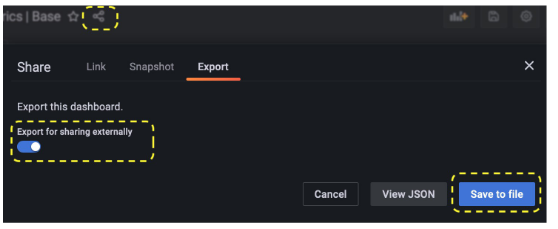
\includegraphics[width=0.6\textwidth]{images/Bloque2/enunciado_grafana.png}
    \label{fig:grafana}
\end{figure}

\subsection*{Solución}

\begin{enumerate}
    \item Primer paso:
    \begin{figure}[H]
        \centering
        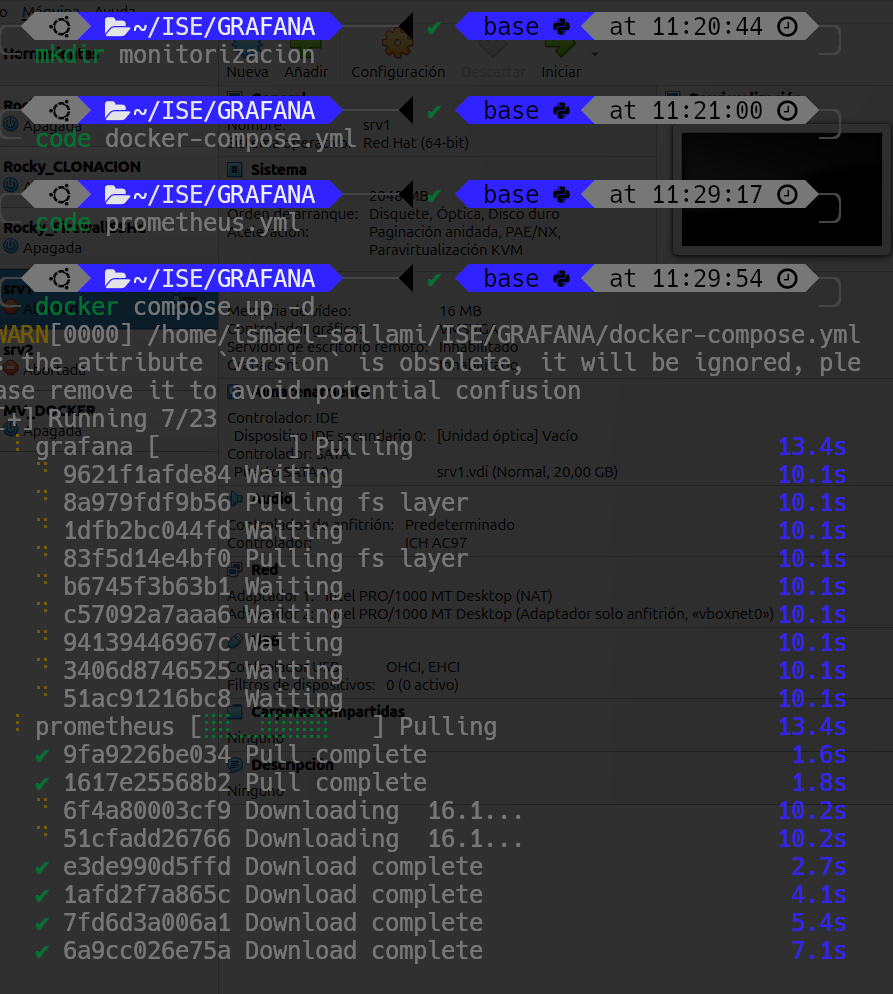
\includegraphics[width=0.6\textwidth]{images/Bloque2/graf1.png}
        \caption{Creación del directorio y descarga de los archivos necesarios}
        \label{fig:instalacion}
    \end{figure}
    \item Clonamos una máquina virtual Rocky Linux. En mi caso le he cambiado la IP y a continuación voy a hacer ssh para hacerlo desde mi máquina local y que me sea más cómodo.
    \item Dentro de la MV Rocky Linux:
    \begin{enumerate}
        \item Primer paso nos bajamos el node-exporter de Prometheus:
        \begin{figure}[H]
            \centering
            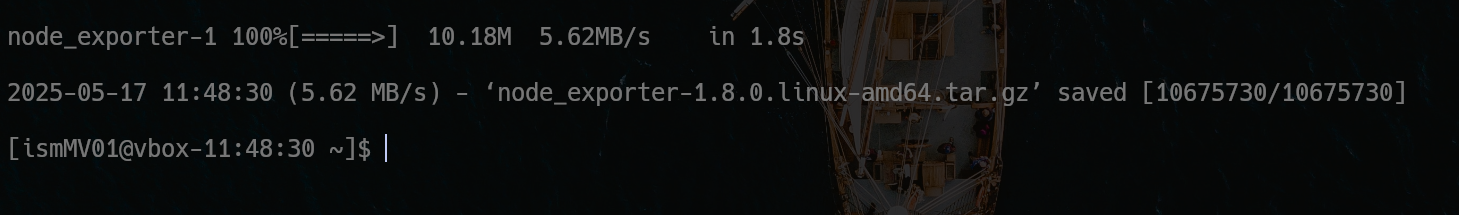
\includegraphics[width=0.6\textwidth]{images/Bloque2/graf2.png}
            \caption{Descarga del node-exporter}
            \label{fig:node-exporter}
        \end{figure}
        \item Descomprimimos el archivo\footnote{He tenido que instalar los comandos tar y wget.}:
        \begin{figure}[H]
            \centering
            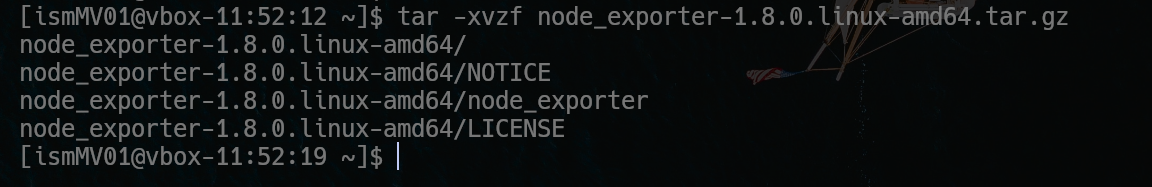
\includegraphics[width=0.6\textwidth]{images/Bloque2/graf3.png}
            \caption{Descompresión del node-exporter}
            \label{fig:descompresion}
        \end{figure}
        \item Movemos el binario al directorio del sistema:
        \begin{figure}[H]
            \centering
            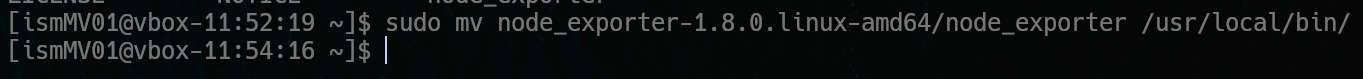
\includegraphics[width=0.6\textwidth]{images/Bloque2/graf4.png}
            \caption{Movimiento del binario al directorio del sistema}
            \label{fig:movimiento}
        \end{figure}
        \item Verificamos que funciona:
        \begin{figure}[H]
            \centering
            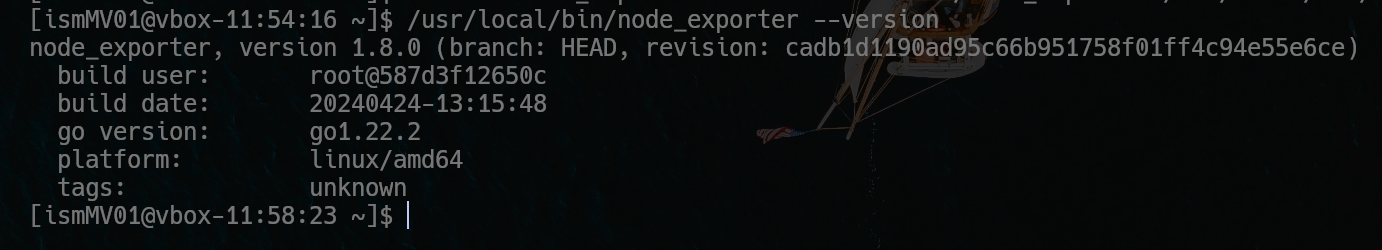
\includegraphics[width=0.6\textwidth]{images/Bloque2/graf5.png}
            \caption{Verificación del funcionamiento del node-exporter}
            \label{fig:verificacion}
        \end{figure}
        \item Creamos el usuario:
        \begin{figure}[H]
            \centering
            
\includegraphics[width=0.6\textwidth]{images/Bloque2/graf6.png}
            \caption{Creación del usuario}
            \label{fig:usuario}
        \end{figure}
        \item Creamos el servicio:
        \begin{figure}[H]
            \centering
            
\includegraphics[width=0.6\textwidth]{images/Bloque2/graf7.png}
            \caption{Creación del servicio}
            \label{fig:servicio}
        \end{figure}
        El contenido del archivo \texttt{node-exporter.service} es el siguiente:
        \begin{lstlisting}[style=customstyle]
            [Unit]
            Description=Node Exporter
            After=network.target

            [Service]
            User=node_exporter
            Group=node_exporter
            Type=simple
            ExecStart=/usr/local/bin/node_exporter

            [Install]
            WantedBy=multi-user.target
        \end{lstlisting}
        \item Recargamos, habilitams y reiniciamos el servicio:
        \begin{figure}[H]
            \centering
            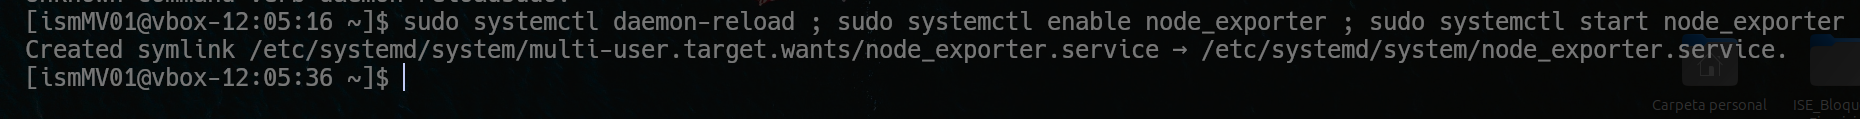
\includegraphics[width=0.6\textwidth]{images/Bloque2/graf8.png}
            \caption{Recarga, habilitación y reinicio del servicio}
            \label{fig:recarga}
        \end{figure}

        \textbf{Se supone que el servicio debería de estar activo, pero me daba un error.} Tras un tiempo intentando arreglarlo, el error se debía a que el servicio node\_exporter fallaba al iniciar debido a una política de SELinux que denegaba su ejecución. Se solucionó corrigiendo el contexto de seguridad SELinux del binario /usr/local/bin/node\_exporter al tipo bin\_t.

        \item Ahora podemos ver que el servicio está activo:
        \begin{figure}[H]
            \centering
            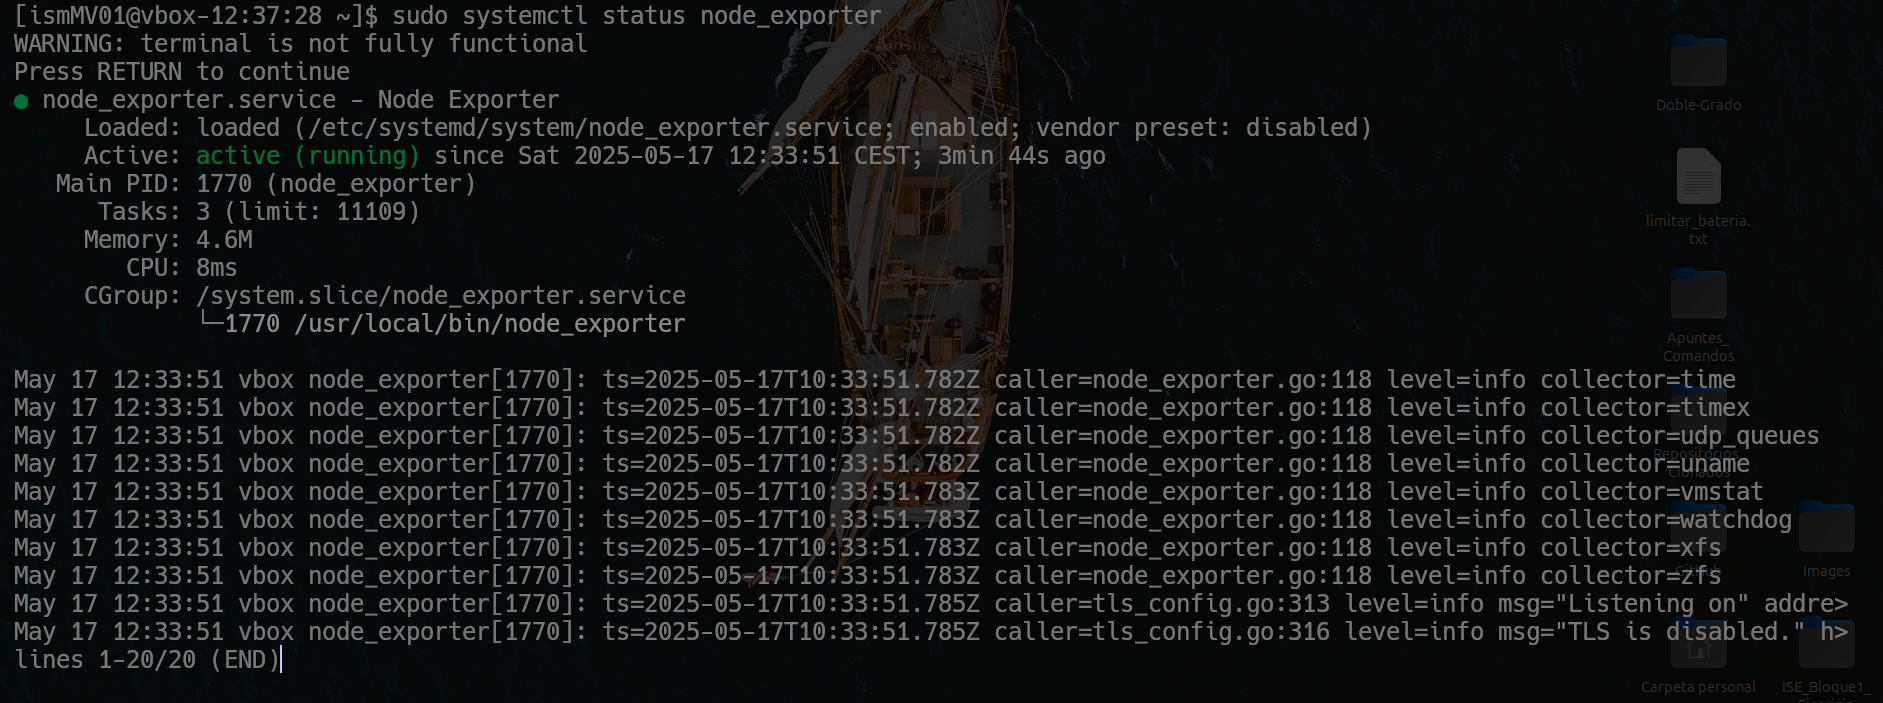
\includegraphics[width=0.6\textwidth]{images/Bloque2/graf9.png}
            \caption{Verificación del servicio}
            \label{fig:verificacion_servicio}
        \end{figure}
        \item Ahora debemos de ver si Node Exporter expone métricas por red, para ello debemos de ejecutar el comando: \micode{curl http://localhost:9100/metrics} en la máquina virtual.
        \begin{figure}[H]
            \centering
            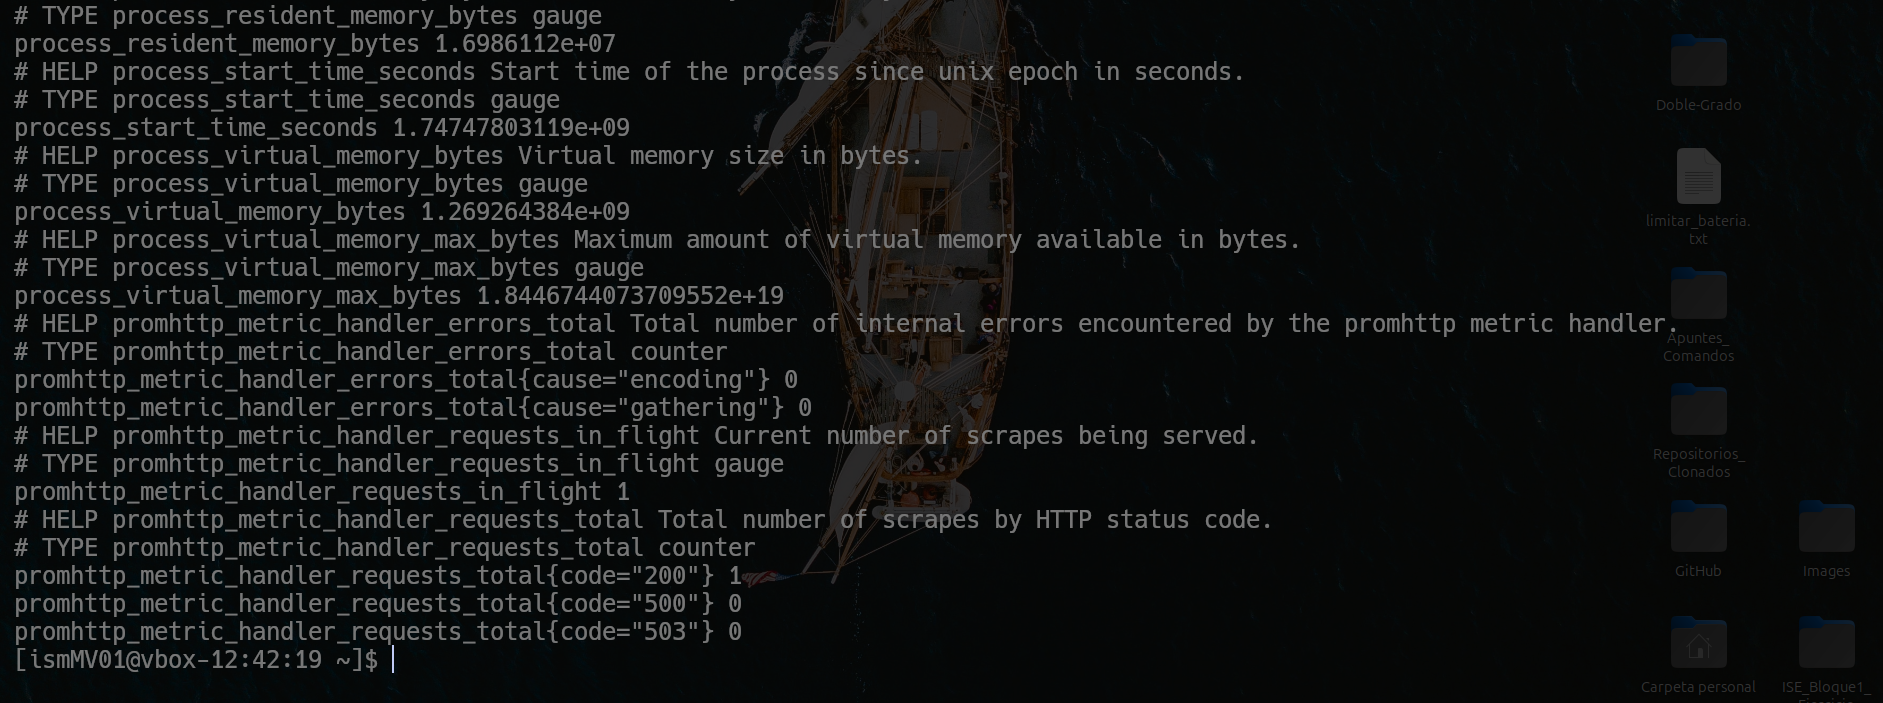
\includegraphics[width=0.6\textwidth]{images/Bloque2/graf10.png}
            \caption{Verificación de las métricas expuestas tras la ejecución del comando}
            \label{fig:metricas}
        \end{figure}
        \item Ahora si accedemos desde nuestra máquina local a la dirección \micode{http://<IP\_VM>:9100/metrics} podemos ver las métricas expuestas por el node-exporter, pero antes debemos de verificar el firewall:
        \begin{figure}[H]
            \centering
            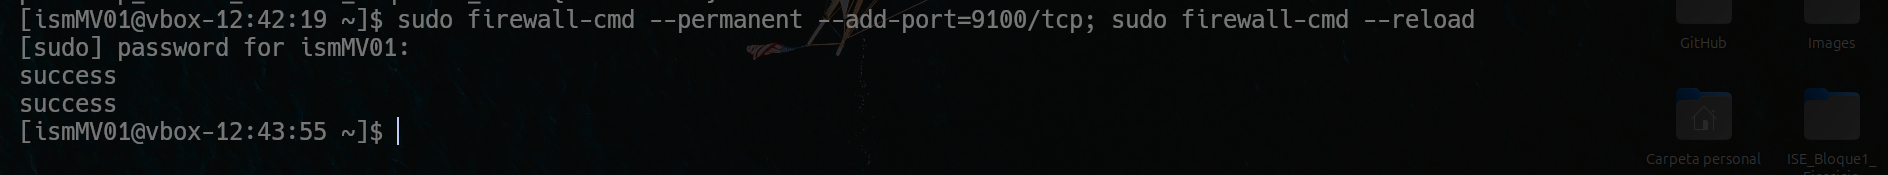
\includegraphics[width=0.6\textwidth]{images/Bloque2/graf11.png}
            \caption{Verificación del firewall}
            \label{fig:firewall}
        \end{figure}
        \item Ahora si accedemos desde nuestra máquina local a la dirección \micode{http://<IP\_VM>:9100/metrics} podemos ver las métricas expuestas por el node-exporter:
        \begin{figure}[H]
            \centering
            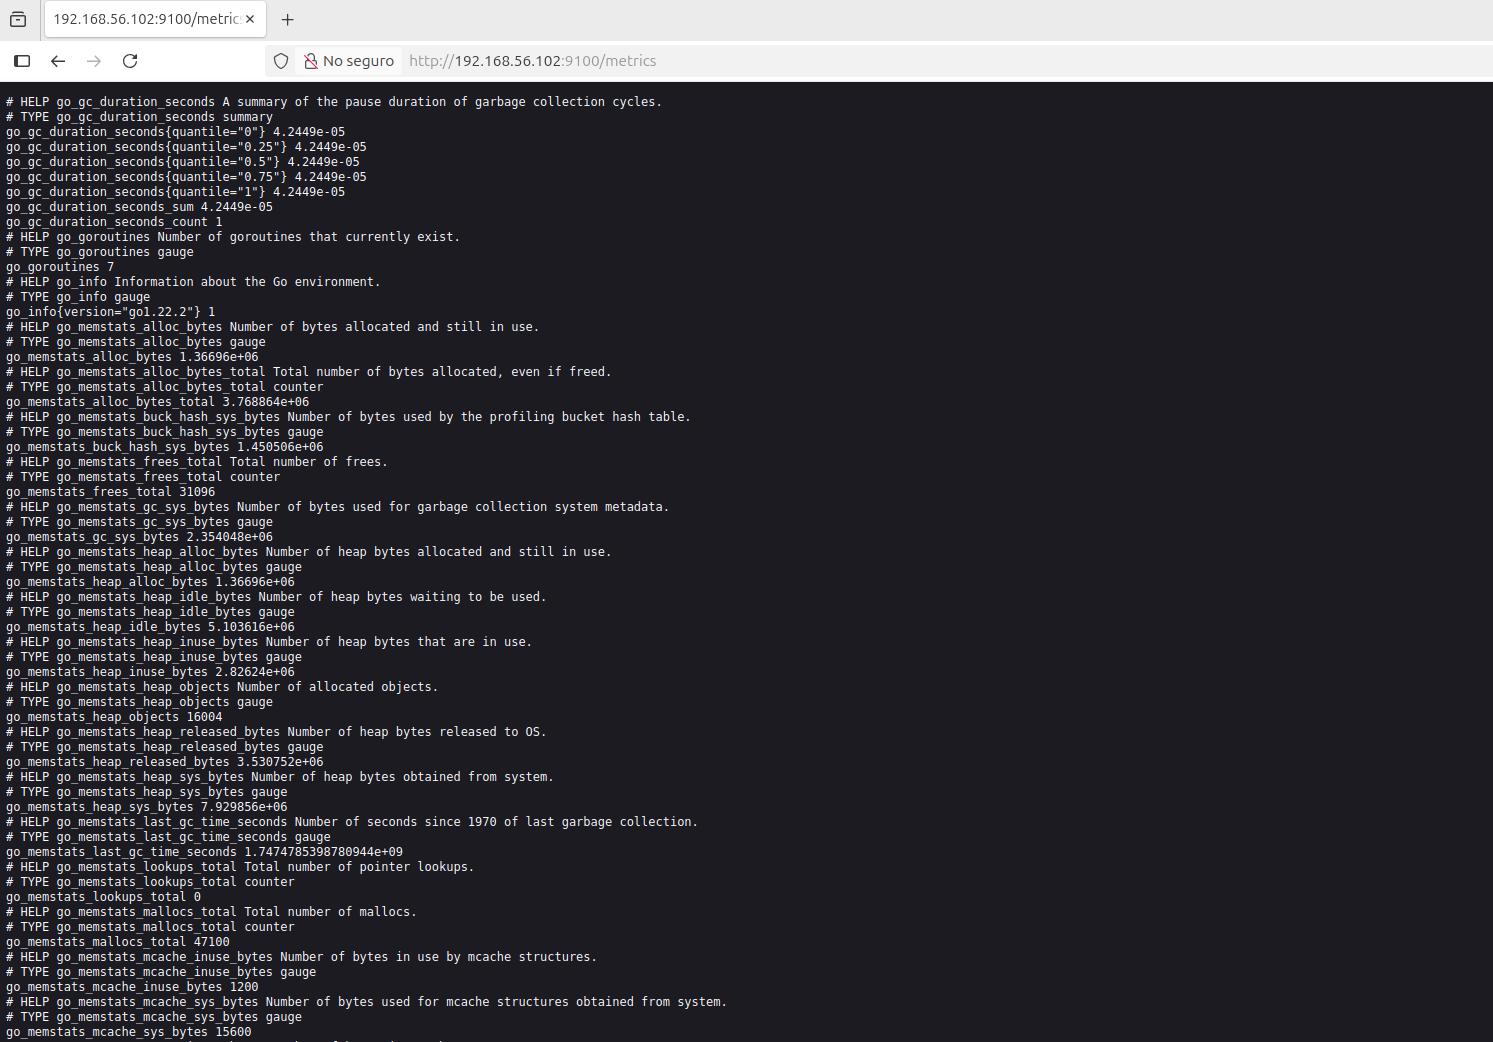
\includegraphics[width=0.6\textwidth]{images/Bloque2/graf12.png}
            \caption{Acceso a las métricas expuestas}
            \label{fig:acceso_metricas}
        \end{figure}

    \end{enumerate}
    \item Ahora debemos de configurar Prometheus para recolectar Métricas de Node Exporter\footnote{Esto lo haremos en nuestra máquina local.}. Para ello debemos de editar el archivo \texttt{prometheus.yml} y añadir el siguiente bloque de configuración:
    \begin{lstlisting}[style=customstyle]
        - job_name: 'rocky_linux_server'
        static_configs:
        - targets: ['192.168.56.102:9100'] 
    \end{lstlisting}
    \item Reiniciamos el contenedor de Prometheus para que recoja la nueva configuración:
    \begin{figure}[H]
        \centering
        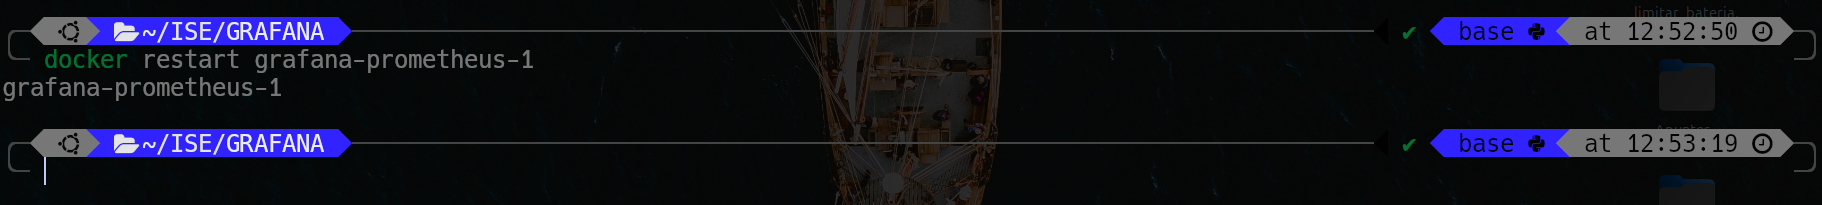
\includegraphics[width=0.6\textwidth]{images/Bloque2/graf13.png}
        \caption{Reinicio del contenedor de Prometheus}
        \label{fig:reinicio}
    \end{figure}
    \textbf{Nota:} Al iniciar los contendores me daba un problema de permisos, por ende, tuve que ejecutar los comandos: 
    \begin{lstlisting}[style=customstyle]
        Para Prometheus:
        Bash

        mkdir -p ./prometheus_data
        sudo chown -R 65534:65534 ./prometheus_data
        sudo chmod -R 755 ./prometheus_data

        Para Grafana:
        Bash

        mkdir -p ./grafana_data
        sudo chown -R 472:472 ./grafana_data
        sudo chmod -R 755 ./grafana_data
    \end{lstlisting}

    Vemos que los contenedores están activos:
    \begin{figure}[H]
        \centering
        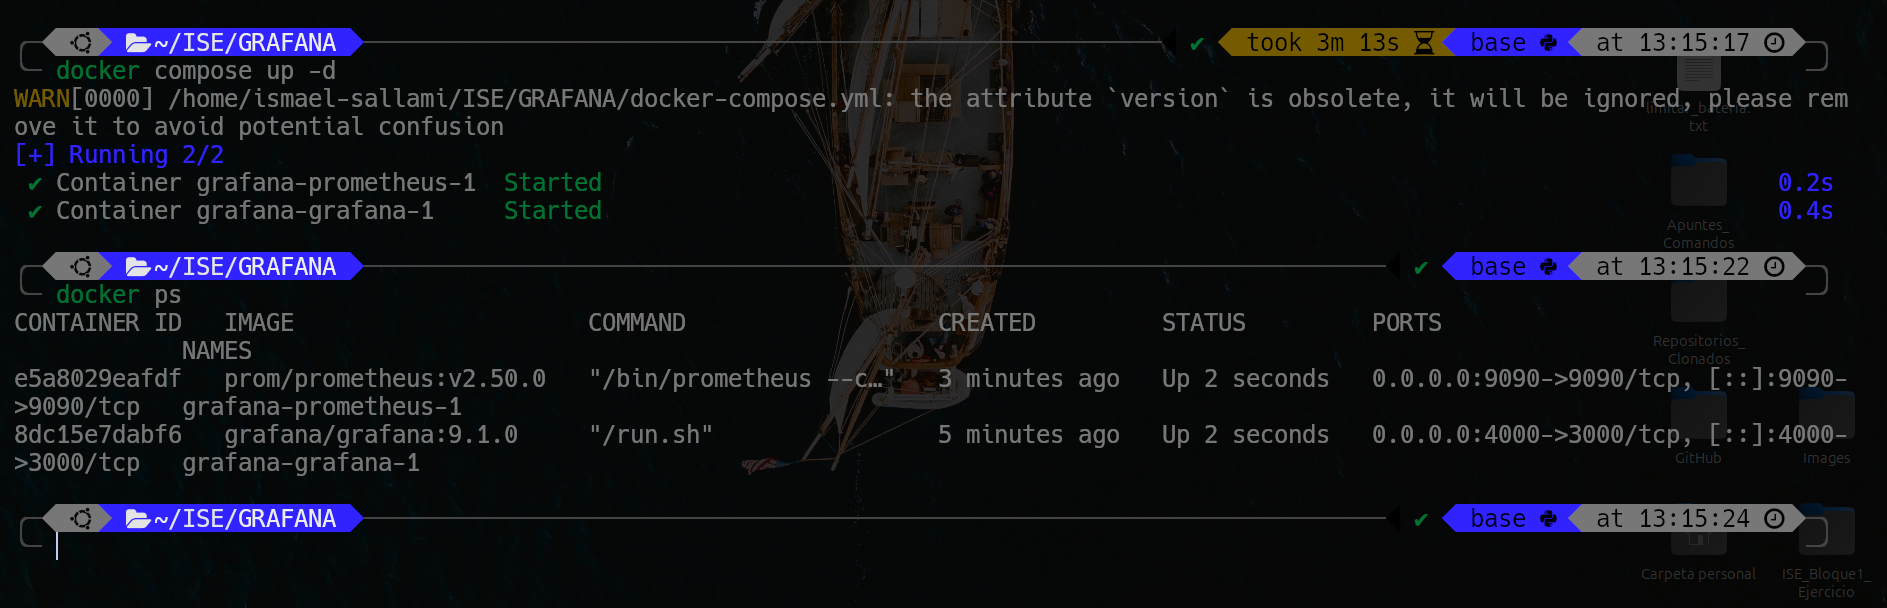
\includegraphics[width=0.6\textwidth]{images/Bloque2/graf14.png}
        \caption{Contenedores activos}
        \label{fig:contenedores}
    \end{figure}
    \item Ahora accedemos a la interfaz web de Prometheus en \micode{http://localhost:9090}:
    \begin{figure}[H]
        \centering
        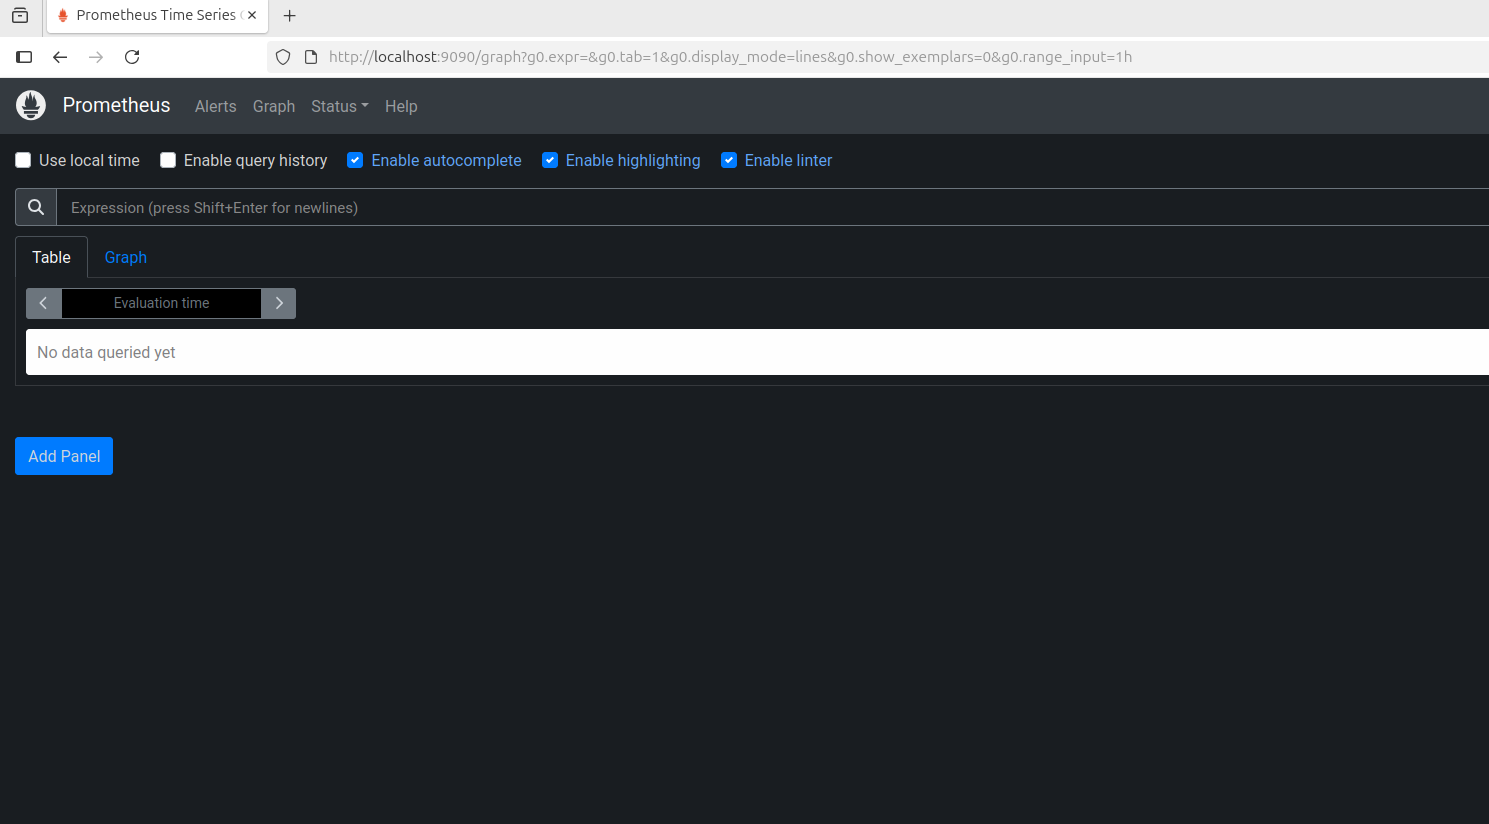
\includegraphics[width=0.6\textwidth]{images/Bloque2/graf15.png}
        \caption{Interfaz web de Prometheus}
        \label{fig:interfaz_prometheus}
    \end{figure}
    \item Vemos que en targets tenemos el Rocky Linux:
    \begin{figure}[H]
        \centering
        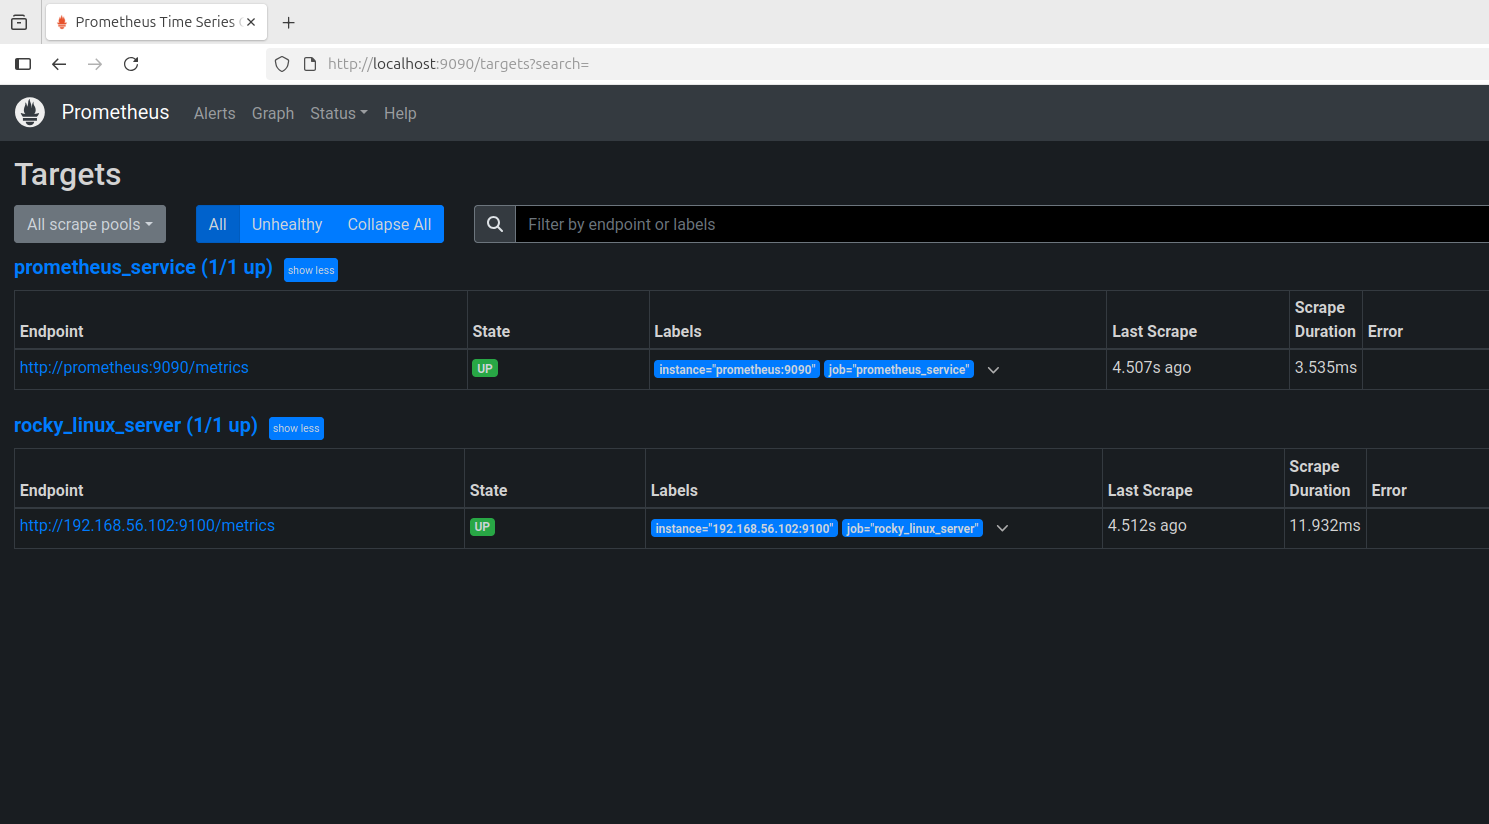
\includegraphics[width=0.6\textwidth]{images/Bloque2/graf16.png}
        \caption{Targets de Prometheus}
        \label{fig:targets}
    \end{figure}
    Vemos que efectivamente está activo ya que el estado es UP.
    \item Ahora accedemos a la interfaz web de Grafana en \micode{http://localhost:4000}:
    \begin{figure}[H]
        \centering
        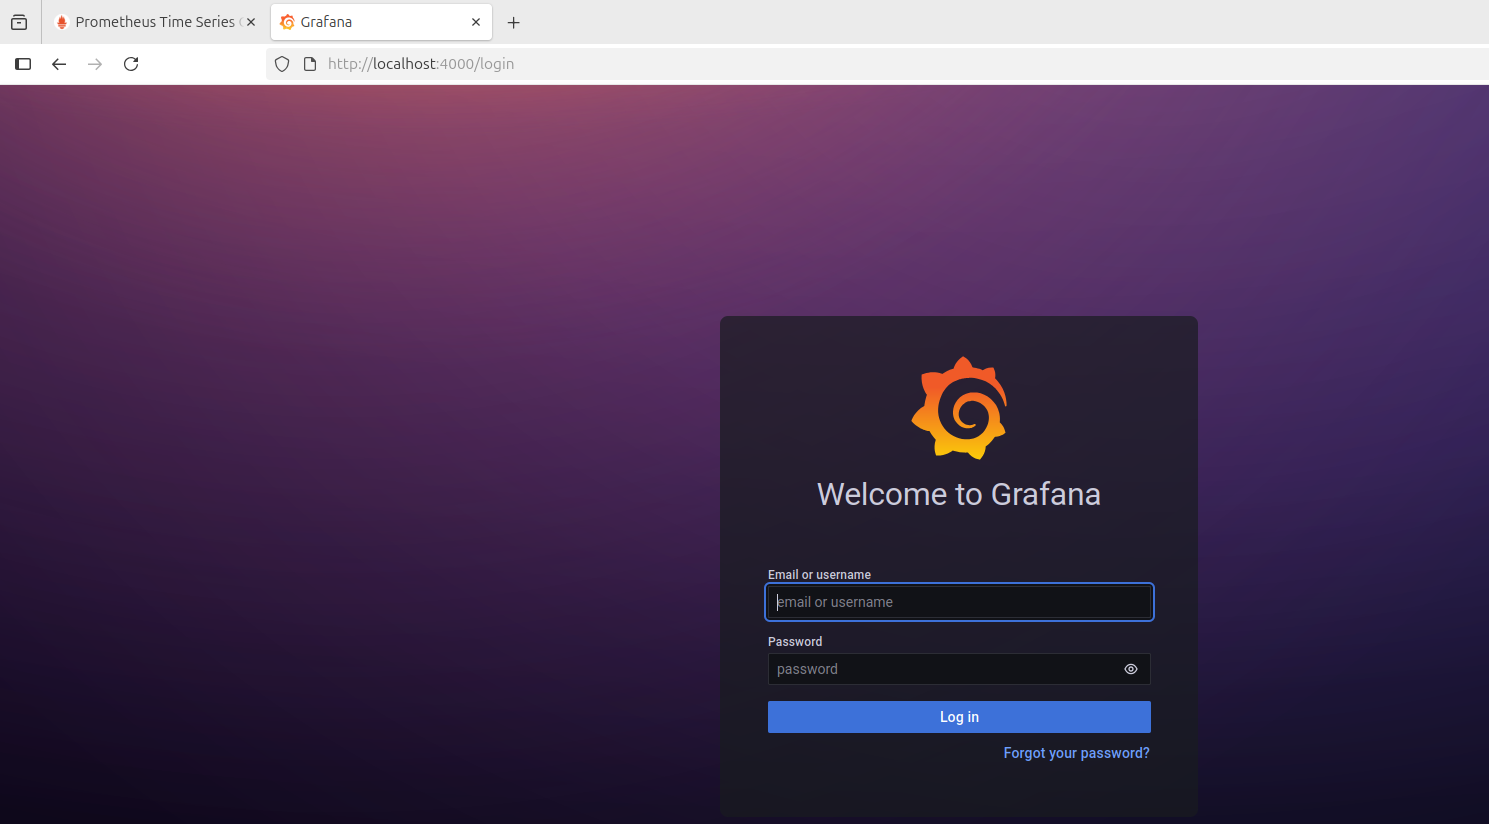
\includegraphics[width=0.6\textwidth]{images/Bloque2/graf17.png}
        \caption{Interfaz web de Grafana}
        \label{fig:interfaz_grafana}
    \end{figure}
    Al ser nuevos, accedemos con el usuario admin y la contraseña admin. Nos pedirá que cambiemos la contraseña, así que la cambiamos.
    \item Ahora debemos de añadir la fuente de datos, para ello vamos a \texttt{Configuration $\rightarrow$ Data Sources $\rightarrow$ Add data source} y seleccionamos Prometheus:
    \begin{figure}[H]
        \centering
        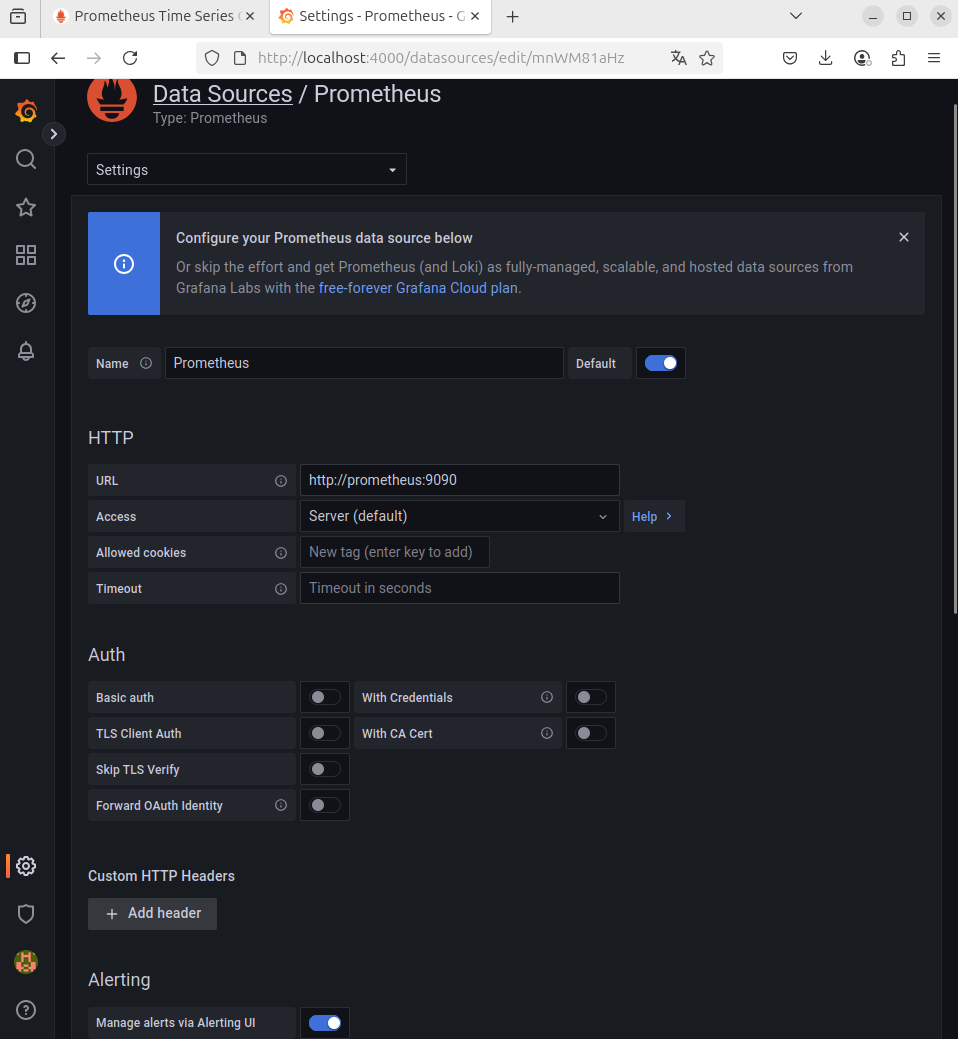
\includegraphics[width=0.6\textwidth]{images/Bloque2/graf18.png}
        \caption{Añadir fuente de datos}
        \label{fig:fuente_datos}
    \end{figure}
    \item Importamos un dashboard de Grafana, para ello vamos a \texttt{Dashboards $\rightarrow$ Import} y buscamos el ID del dashboard que queremos importar. En mi caso he elegido el ID 1860\footnote{\url{https://grafana.com/grafana/dashboards/1860}}:
    \begin{figure}[H]
        \centering
        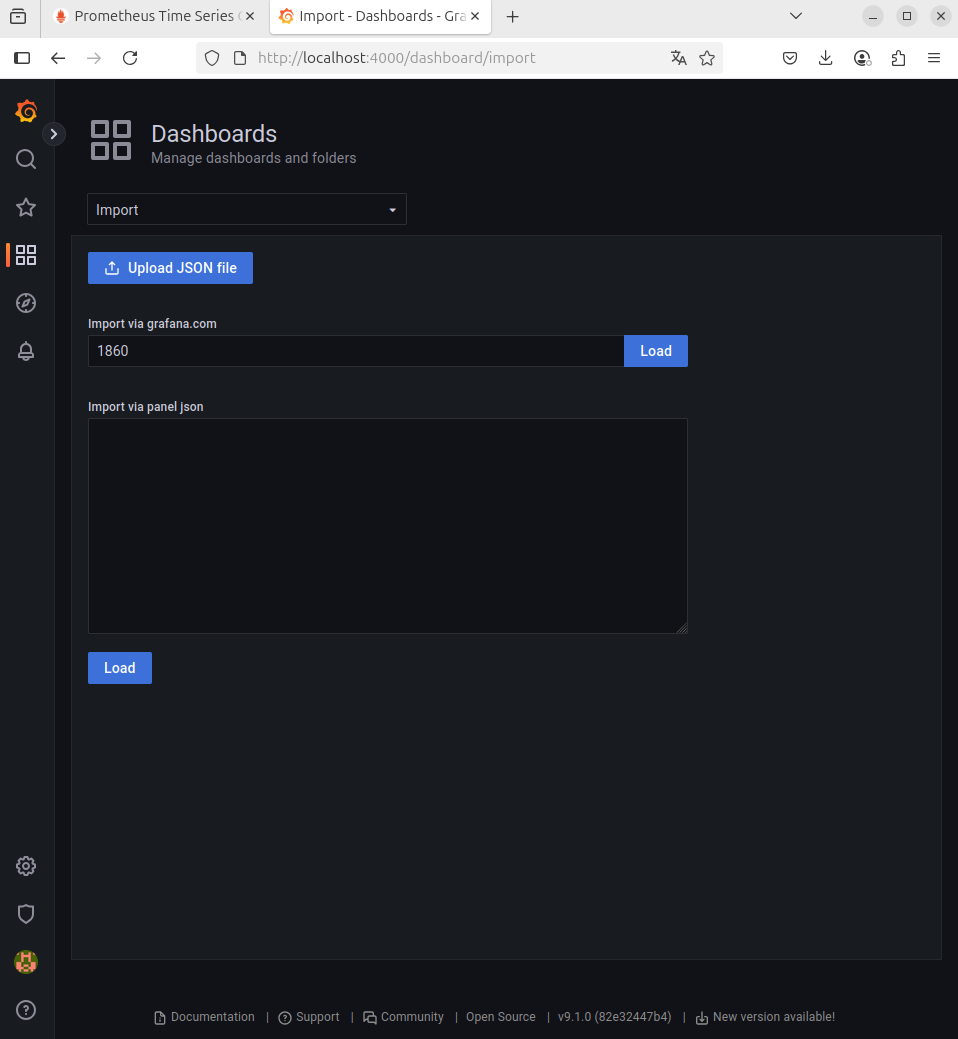
\includegraphics[width=0.6\textwidth]{images/Bloque2/graf19.png}
        \caption{Importación del dashboard}
        \label{fig:importacion_dashboard}
    \end{figure}
    \item Ahora debemos de añadir las iniciales a los paneles, quedando de esta manera(las iniciales son ISM):
    \begin{figure}[H]
        \centering
        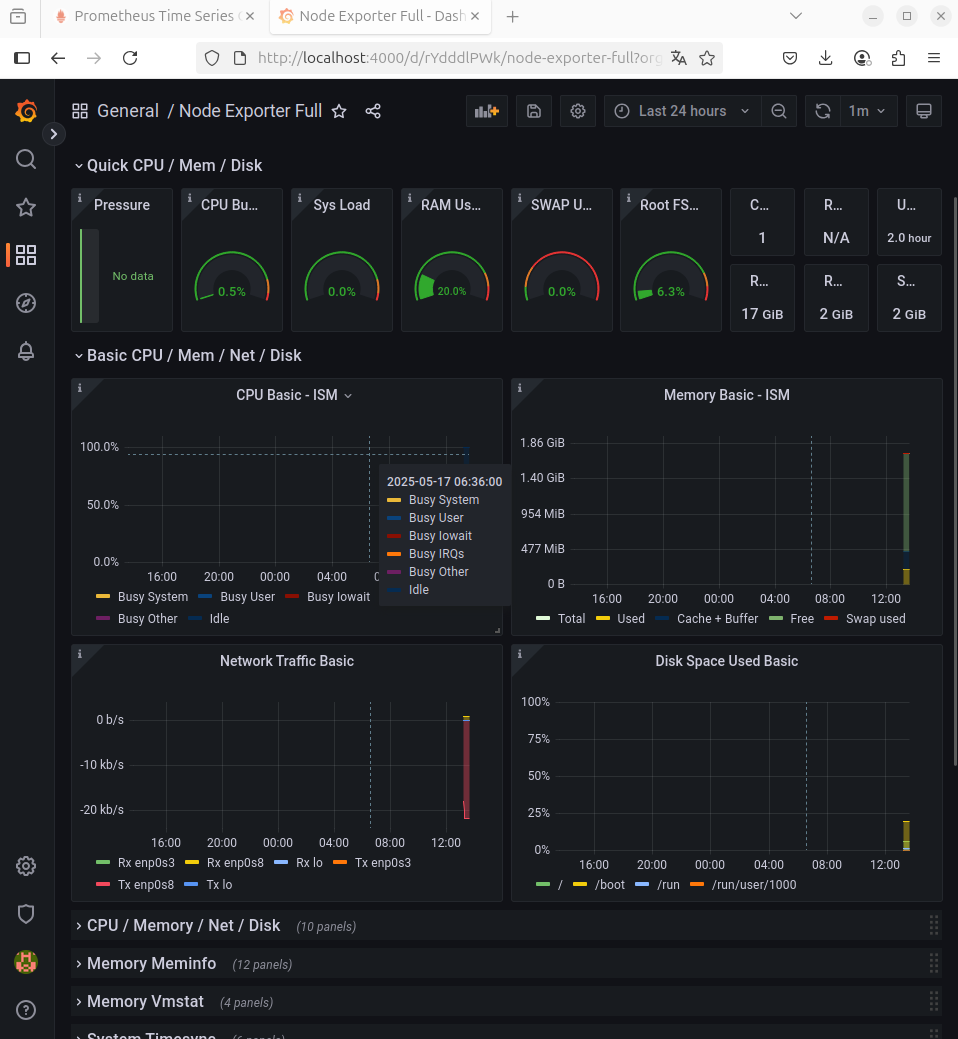
\includegraphics[width=0.6\textwidth]{images/Bloque2/graf20.png}
        \caption{Añadido de las iniciales a los paneles}
        \label{fig:iniciales_paneles}
    \end{figure} 
    Siguiendo con el enunciado vamos a responder a la parte de:
    ``El dashboard debe recibir como identificador, el nombre y apellidos del alumno/a en CamelCase
    junto con el sufijo “Linux”. Por ejemplo, mariaGarciaPerezLinux. Todos los paneles creados se
    presentarán con un título que contenga las iniciales del alumno/a. Siguiendo con el ejemplo
    anterior: \%CPU (MGP).''
    De manera que el dashboard quedaría de la siguiente manera:
    \begin{figure}[H]
        \centering
        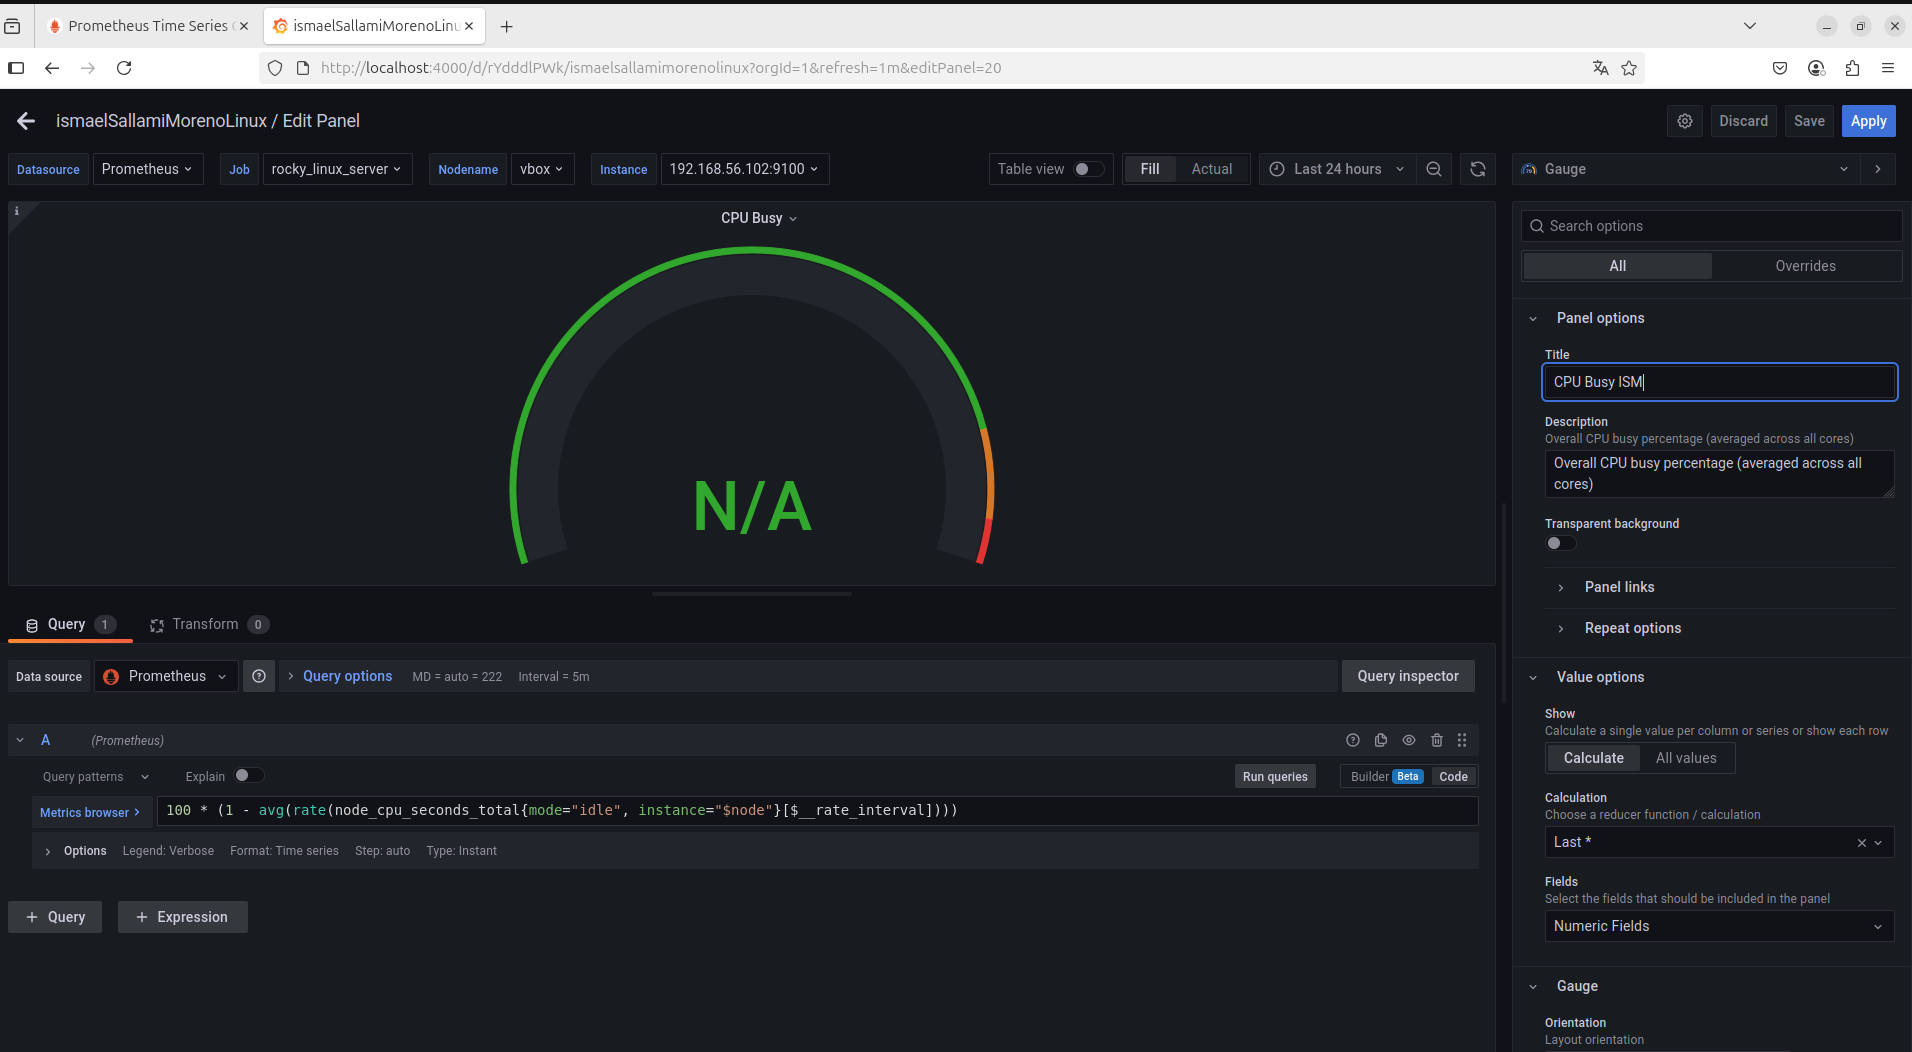
\includegraphics[width=0.6\textwidth]{images/Bloque2/graf21.png}
        \caption{Dashboard con el nombre y apellidos del alumno}
        \label{fig:dashboard}
    \end{figure}
    Como vemos en la imagen el dashboard tiene el nombre y apellidos del alumno/a en CamelCase junto con el sufijo “Linux” y todos los paneles creados se presentan con un título que contiene las iniciales del alumno/a (esto se omite ya que al ser un dashboard predefinido tiene varios paneles y es muy costoso ir cambiando todos los nombres de los paneles).
    \item Añadimos un nuevo panel en este dashboard que hemos creado con nuestro nombre:
    \begin{figure}[H]
        \centering
        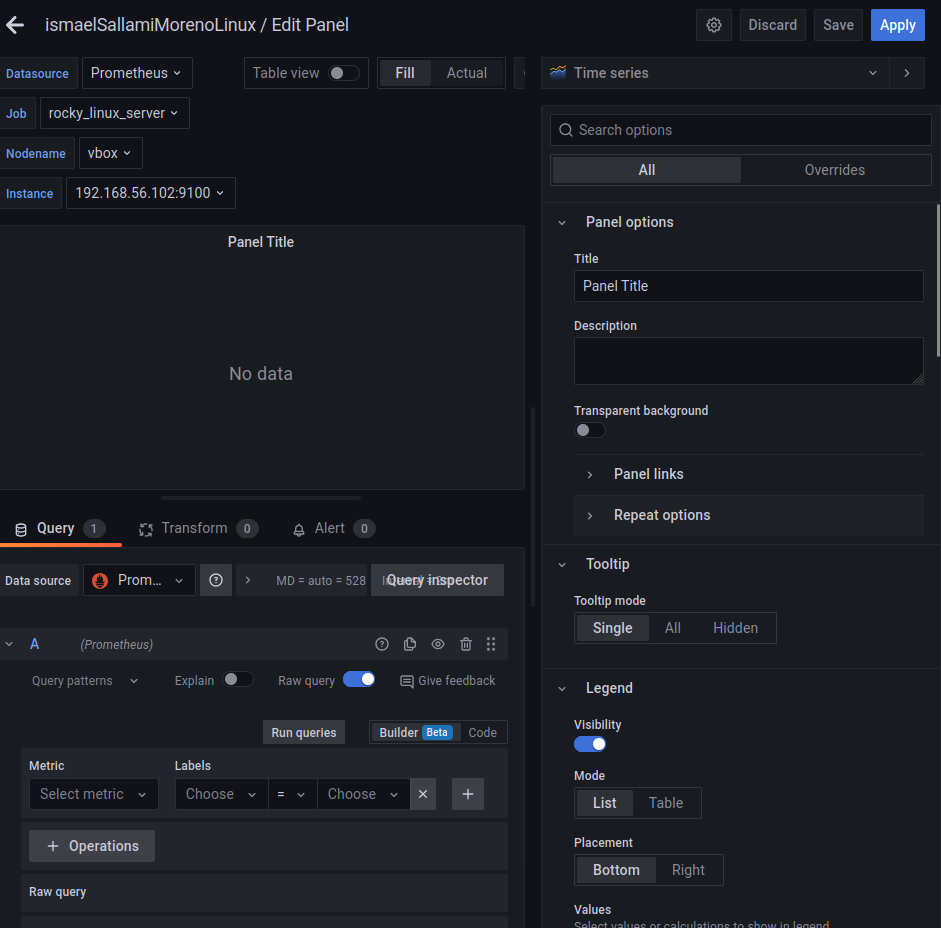
\includegraphics[width=0.6\textwidth]{images/Bloque2/graf22.png}
        \caption{Añadido de un nuevo panel}
        \label{fig:nuevo_panel}
    \end{figure}
    Al añadir el panel del ssh no me daba los valores correctos, así que probé a poner la métrica en el prometheus y tampoco me daba resultado, por ende añadí al fichero \texttt{/etc/systemd/system/node\_exporter.service}
    a la línea de ``exec'' la parte de \micode{--collector.systemd} y recargando toda la configuración sí me da el resultado correcto. Nos quedaría de la siguiente manera:
    \begin{figure}[H]
        \centering
        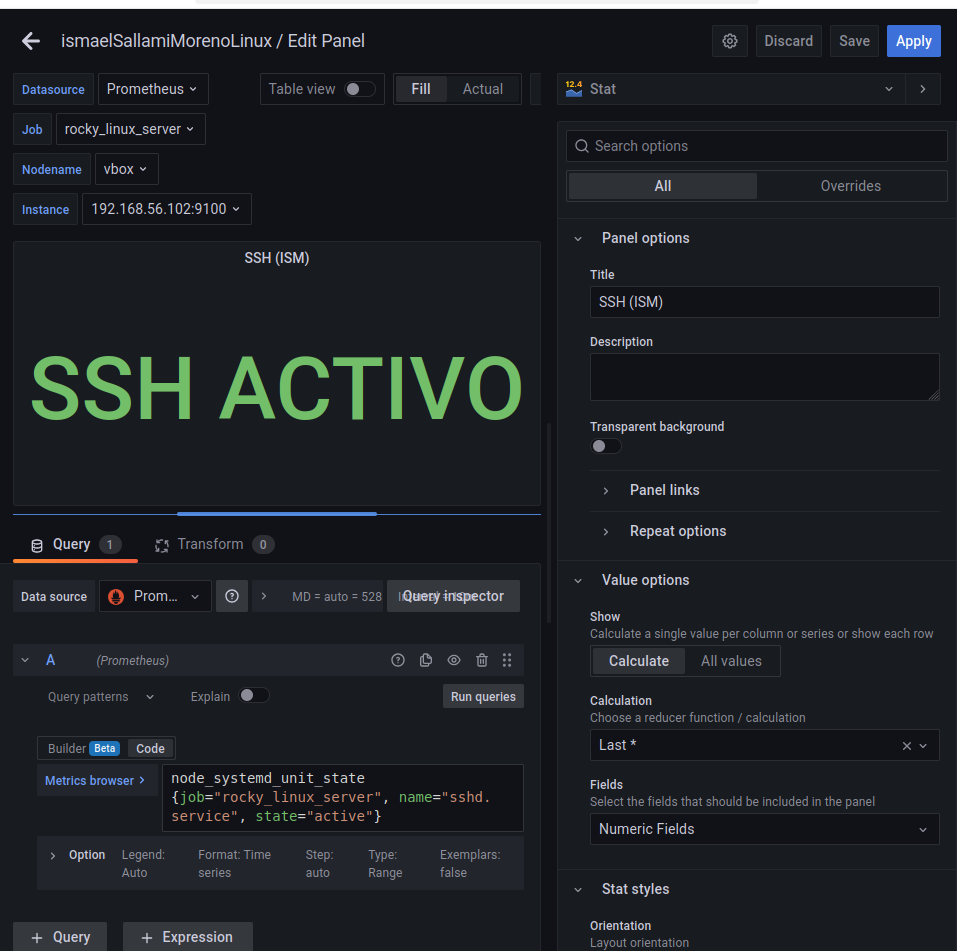
\includegraphics[width=0.6\textwidth]{images/Bloque2/graf23.png}
        \caption{Añadido del panel del ssh}
        \label{fig:panel_ssh}
    \end{figure}

    \item Ahora debemos de hacer lo mismo para httpd:
    \begin{figure}[H]
        \centering
        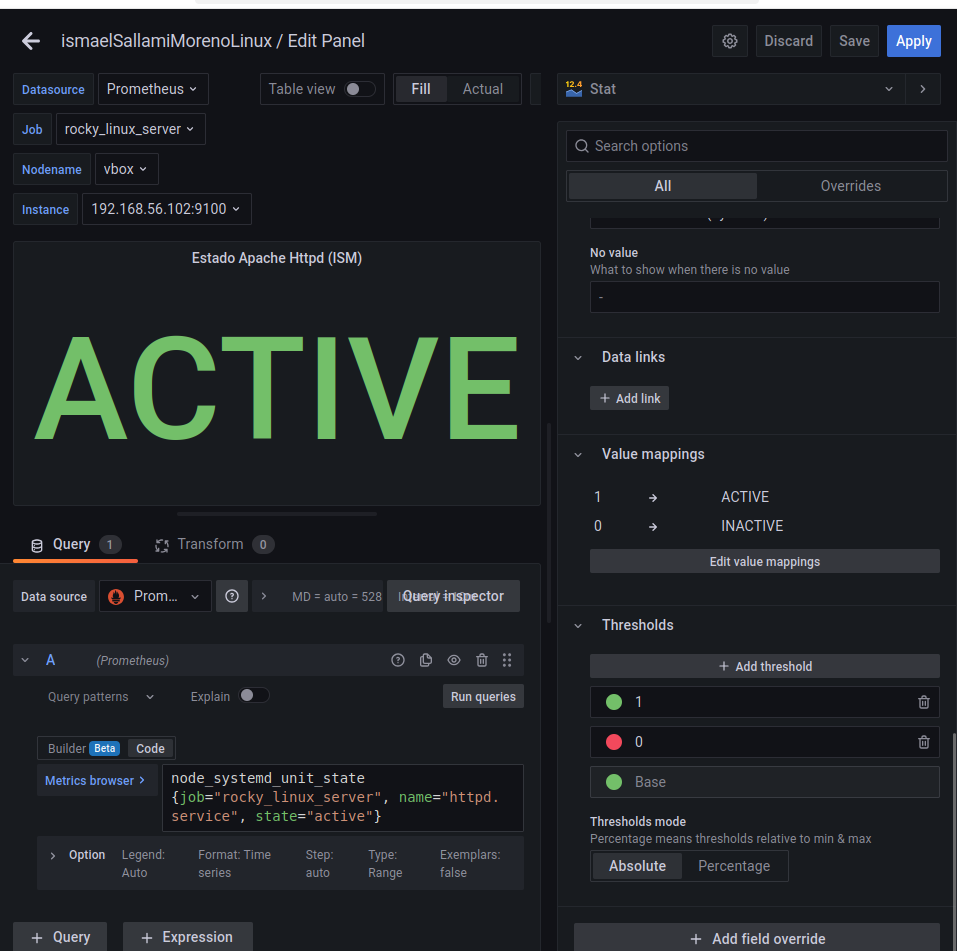
\includegraphics[width=0.6\textwidth]{images/Bloque2/graf24.png}
        \caption{Añadido del panel del httpd}
        \label{fig:panel_httpd}
    \end{figure}

    De manera conjunta nos quedaría de la siguiente manera:
    \begin{figure}[H]
        \centering
        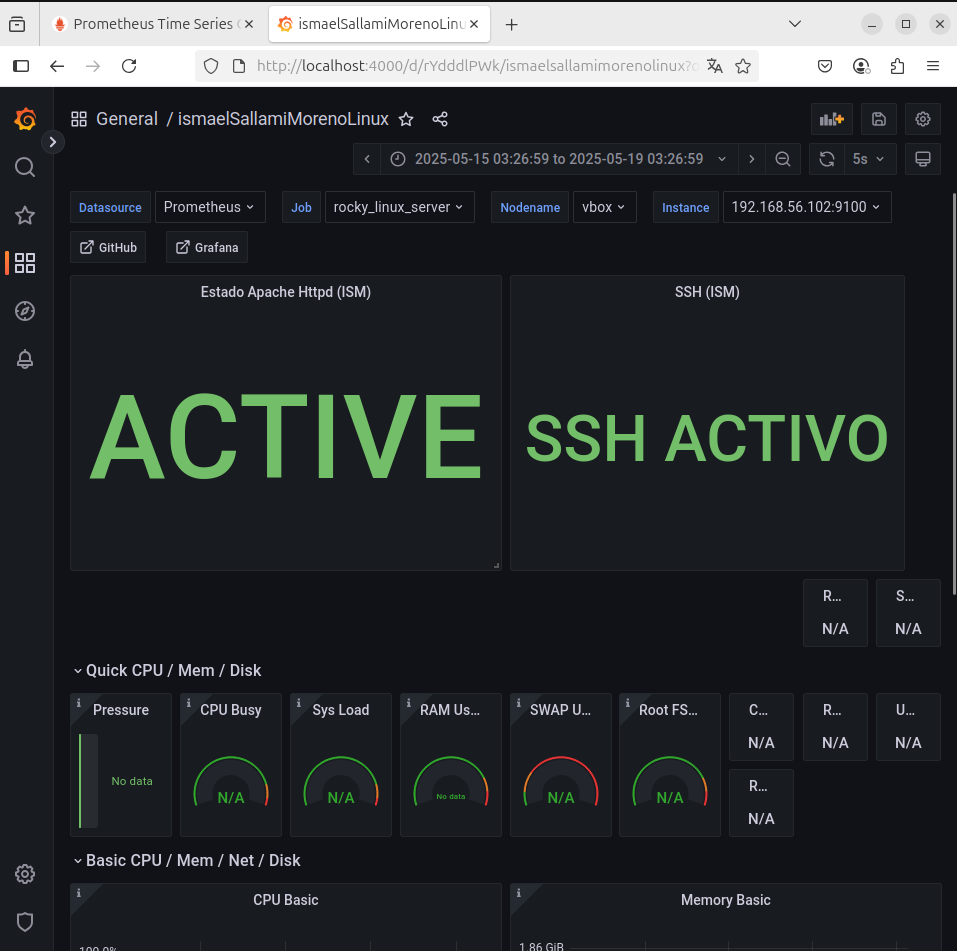
\includegraphics[width=0.6\textwidth]{images/Bloque2/graf25.png}
        \caption{Añadido de los paneles del ssh y httpd}
        \label{fig:paneles_ssh_httpd}
    \end{figure}
    \textbf{Nota:} Las expresiones regulares que he utilizado para el ssh y httpd aparecen en las imágenes de arriba.
    \item Ahora añadimos el panel de la CPU:
    \begin{figure}[H]
        \centering
        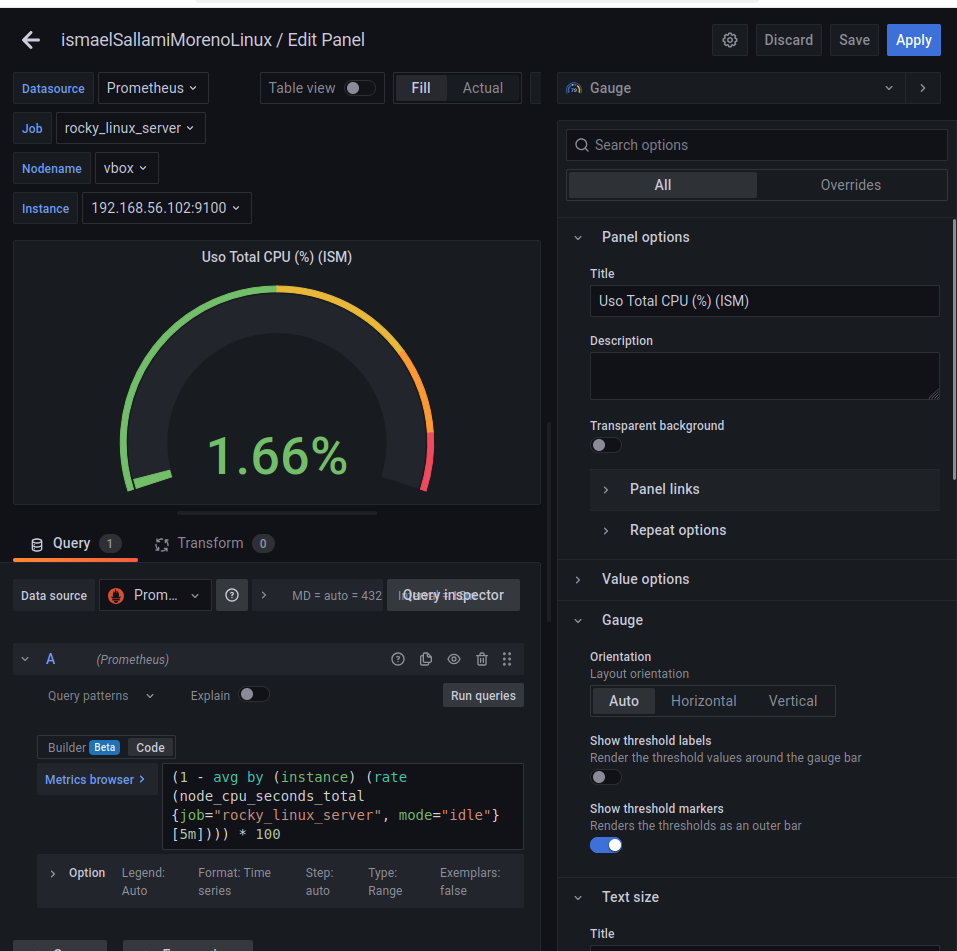
\includegraphics[width=0.6\textwidth]{images/Bloque2/graf26.png}
        \caption{Añadido del panel de la CPU}
        \label{fig:panel_cpu}
    \end{figure}

    \item Ahora añadimos la alarma al panel de la CPU:
    \begin{figure}[H]
        \centering
        \begin{minipage}{0.45\textwidth}
            \centering
            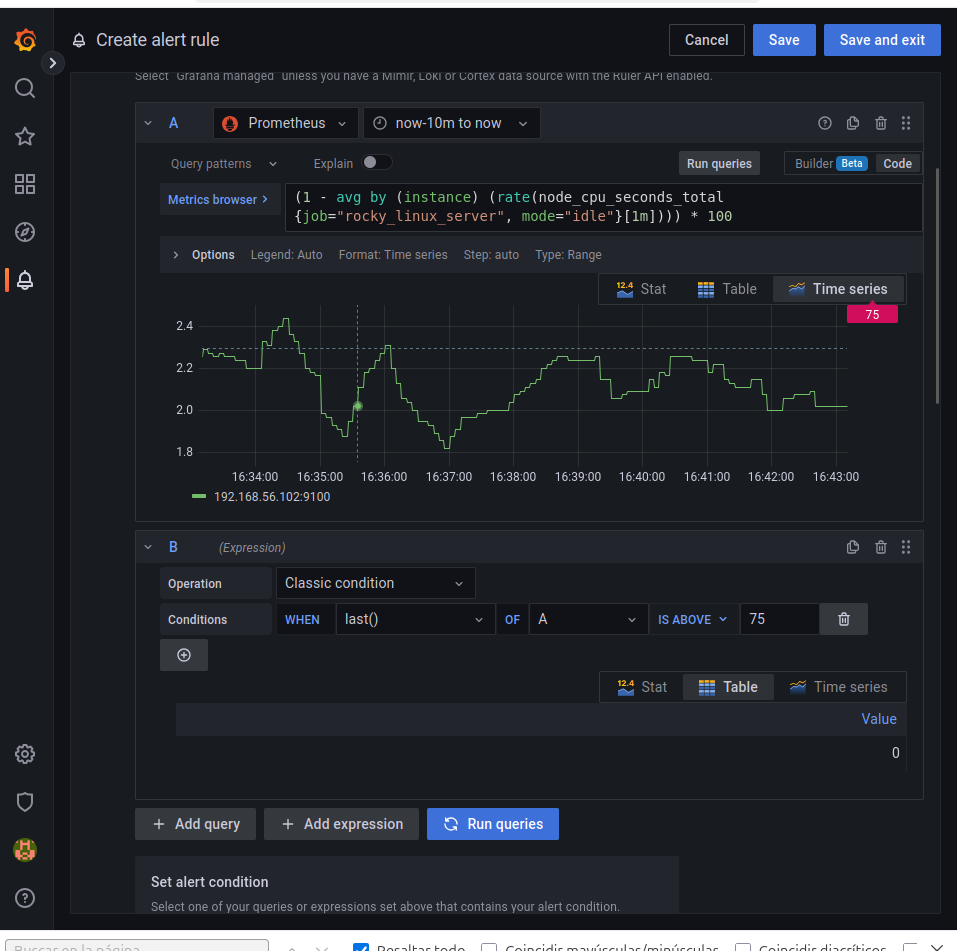
\includegraphics[width=\textwidth]{images/Bloque2/graf27.png} % Llave añadida
            \caption{Primera Parte de la alarma}
            \label{fig:image1graf}
        \end{minipage}
        \hfill
        \begin{minipage}{0.45\textwidth}
            \centering
            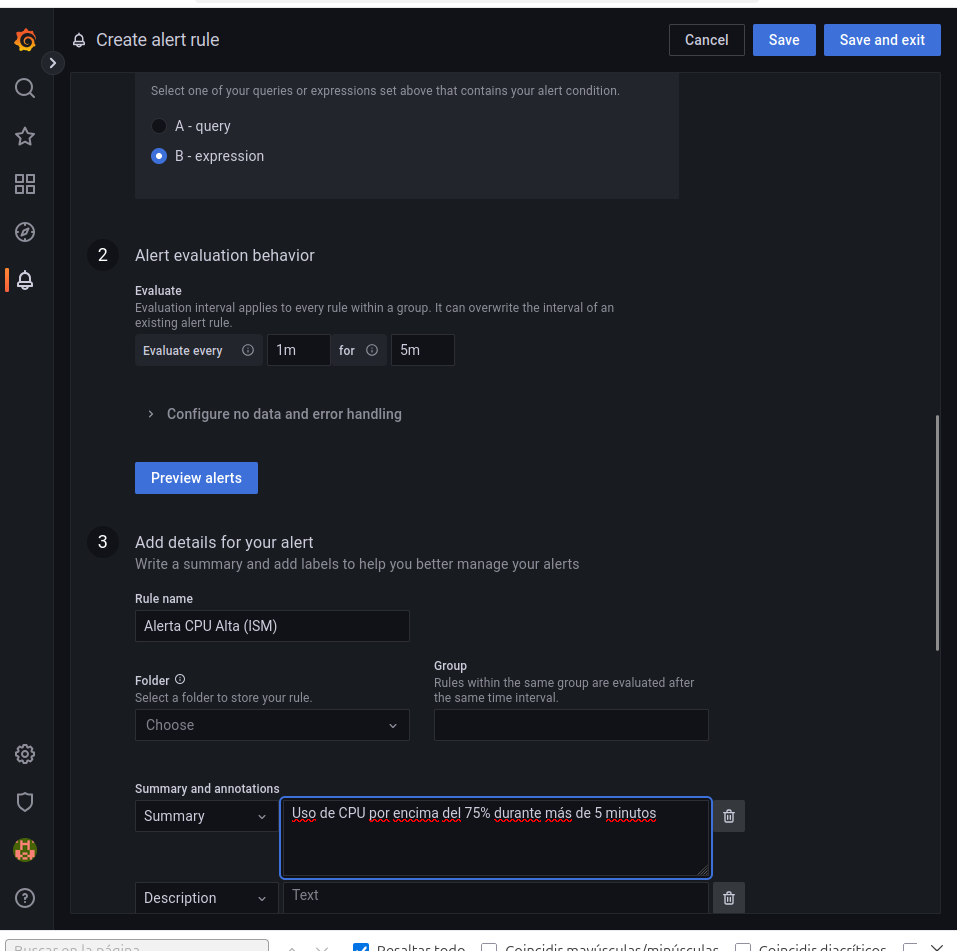
\includegraphics[width=\textwidth]{images/Bloque2/graf28.png}
            \caption{Segunda Parte de la alarma}
            \label{fig:image2graf}
        \end{minipage}
    \end{figure}
    \item De manera que la alarma nos quedaría de la siguiente manera:
    \begin{figure}[H]
        \centering
        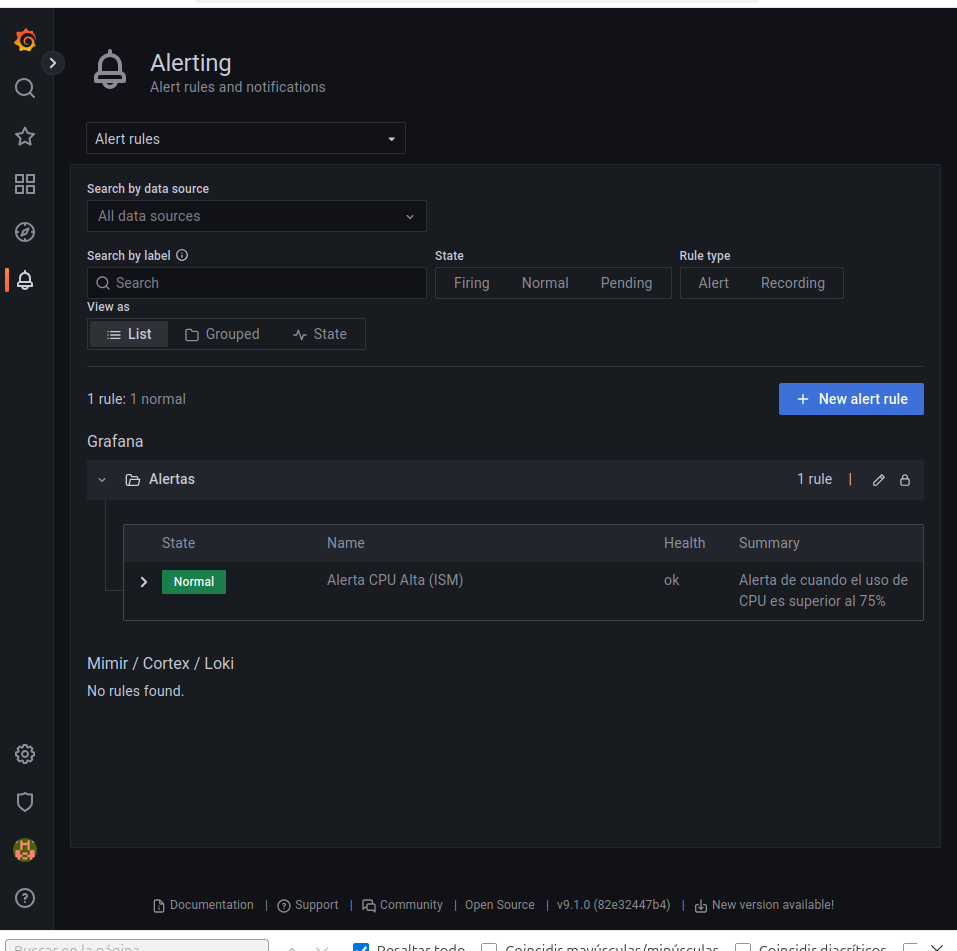
\includegraphics[width=0.6\textwidth]{images/Bloque2/graf29.png}
        \caption{Alarma de la CPU}
        \label{fig:alarma_cpu}
    \end{figure}
    \item Ahora vamos a ver el estado incial y el estado final de la CPU.
    \begin{figure}[H]
        \centering
        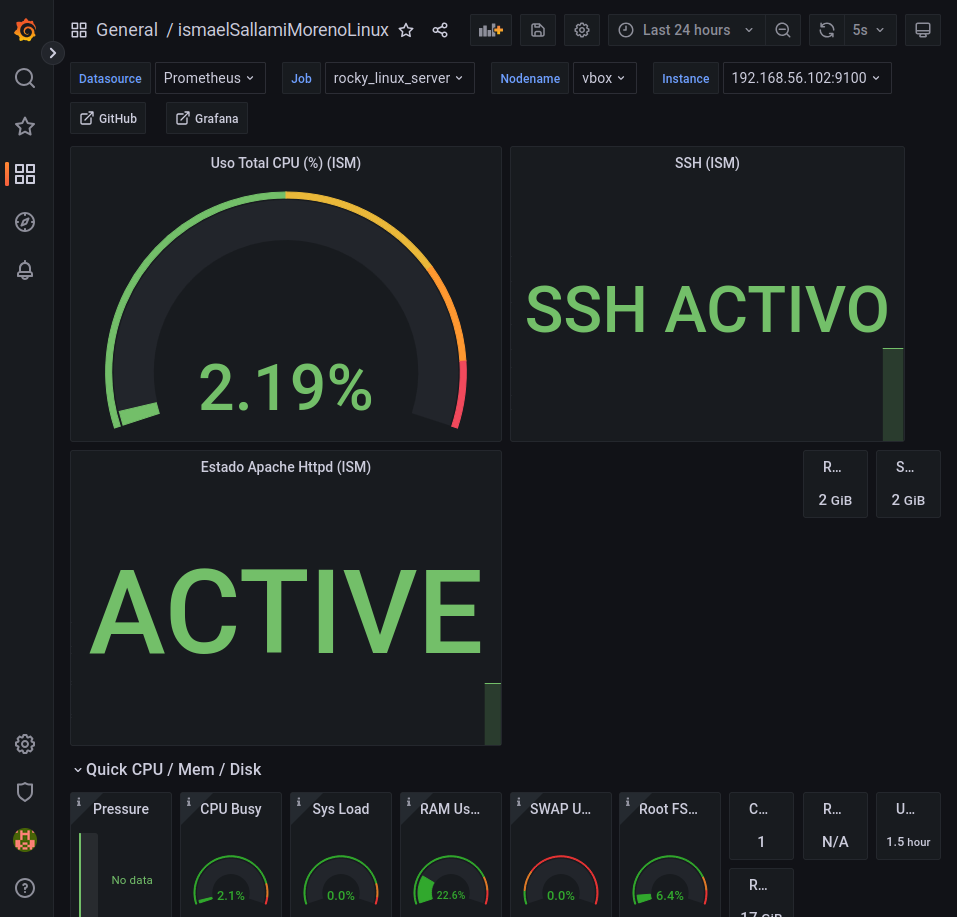
\includegraphics[width=0.6\textwidth]{images/Bloque2/graf30.png}
        \caption{Estado inicial de la CPU}
        \label{fig:estado_inicial_cpu}
    \end{figure}

    Para instalar el stress en la máquina virtual de Rocky Linux, ejecutamos el siguiente comando:
    \begin{lstlisting}[style=customstyle]
    sudo dnf install epel-release -y
    sudo dnf makecache
    sudo dnf install stress -y
    \end{lstlisting}

    Vemos que si ejecutamos el comando \micode{stress --cpu 1 --timeout 360s} la carga en grafana va a subir poco a poco y cuando supere el 75\% de CPU durante 5 minutos se disparará la alarma:
    \begin{figure}[H]
        \centering
        \begin{minipage}{0.45\textwidth}
            \centering
            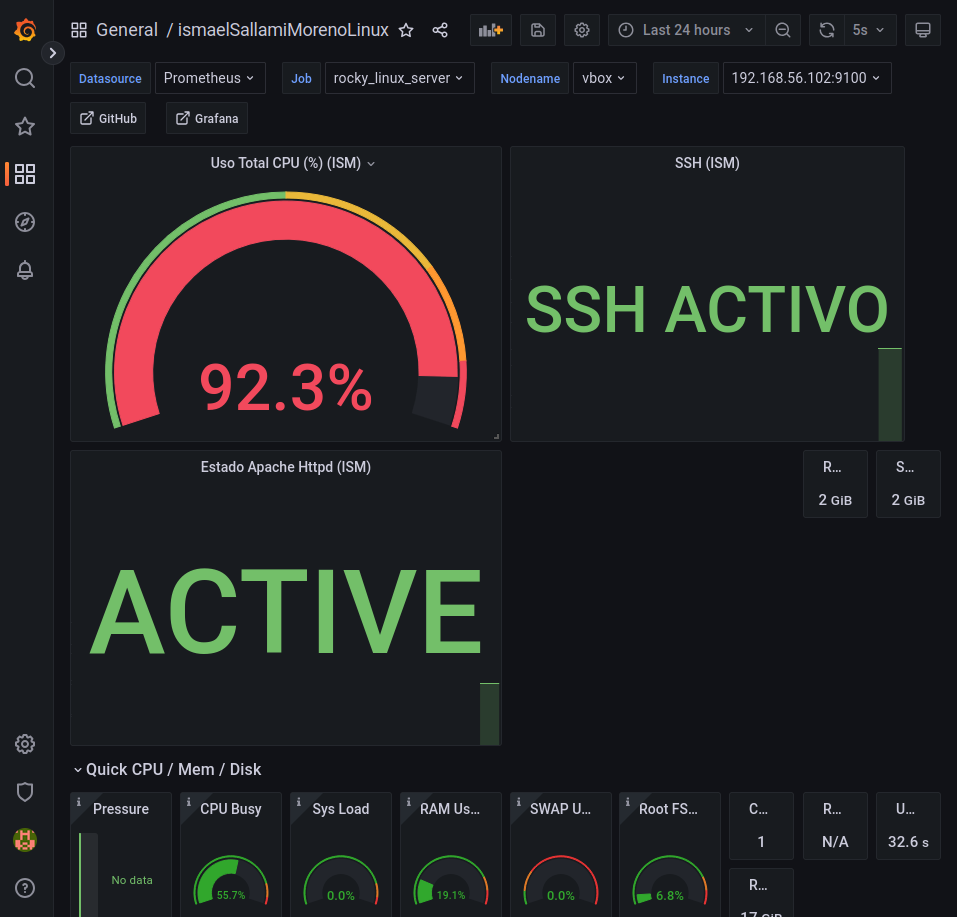
\includegraphics[width=\textwidth]{images/Bloque2/graf31.png}
            \caption{Alto uso de CPU gracias al stress}
            \label{fig:image1}
        \end{minipage}
        \hfill
        \begin{minipage}{0.45\textwidth}
            \centering
            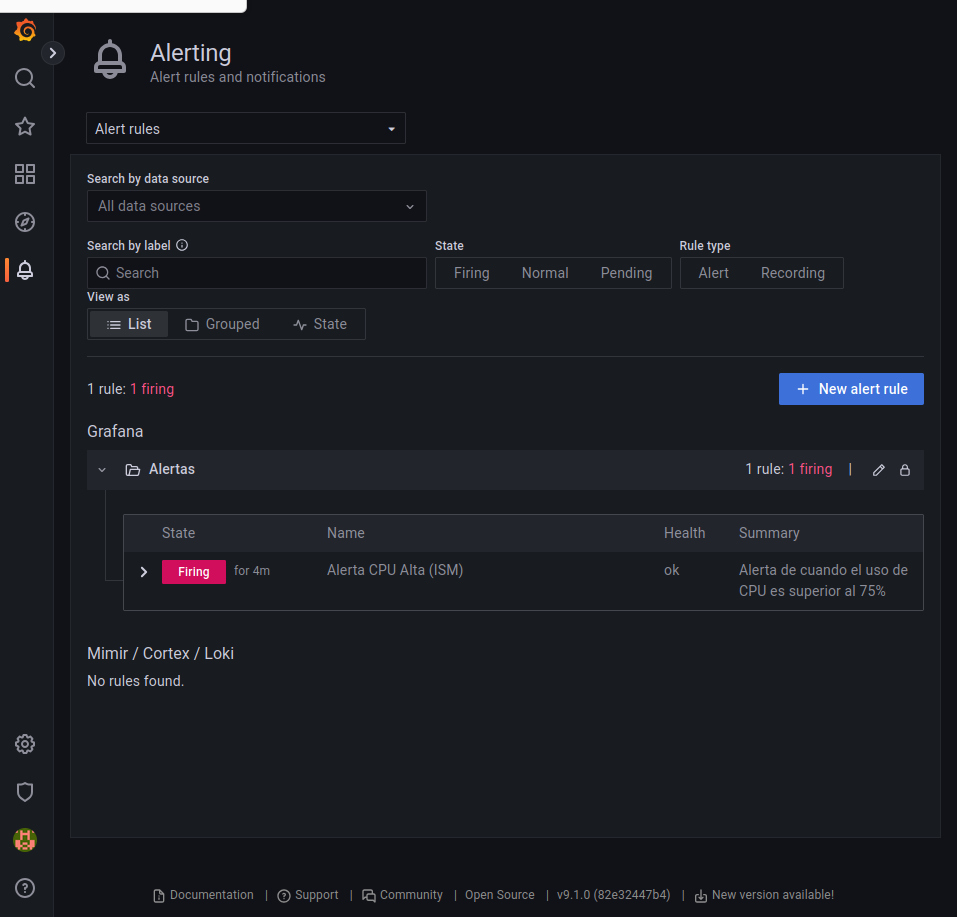
\includegraphics[width=\textwidth]{images/Bloque2/graf33.png}
            \caption{Disparo de la alarma}
            \label{fig:image2}
        \end{minipage}
    \end{figure}

    Luego al cancelar el stress, la carga de CPU baja y la alarma se apaga:
    \begin{figure}[H]
        \centering
        \begin{minipage}{0.45\textwidth}
            \centering
            \includegraphics[width=\textwidth]{images/Bloque2/graf32.png}
            \caption{Vuelta al uso normal de CPU}
            \label{fig:image1}
        \end{minipage}
        \hfill
        \begin{minipage}{0.45\textwidth}
            \centering
            \includegraphics[width=\textwidth]{images/Bloque2/graf34.png}
            \caption{Estado normal de la alarma}
            \label{fig:image2}
        \end{minipage}
    \end{figure}
    
    El comando ha sido:
    \begin{figure}[H]
        \centering
        \includegraphics[width=0.6\textwidth]{images/Bloque2/graf35.png}
        \caption{Comando de stress}
        \label{fig:comando_stress}
    \end{figure}
\end{enumerate}

\textcolor{blue}{Ahora pasamos a la parte de la resolución de la API WEB.}

Para la realización de esta parte debemos de tener en cuenta el ejercicio de prueba de carga con JMETER, para ello lanzamos el contenedor de la API Web y entramos en la url \micode{http://localhost:3000/metrics}.

Una vez añadido los paneles y demás \footnote{A continuación se adjuntan las expresiones regulares que he utilizado para cada uno de los paneles.}, vamos a ver como queda el antes y después de los paneles tras la carga de JMeter.

\begin{figure}[H]
    \centering
    \includegraphics[width=0.6\textwidth]{images/Bloque2/graf36.png}
    \caption{Paneles de la API Web Antes de la carga}
    \label{fig:paneles_api}
\end{figure}

Por último, tras la carga de JMeter, los paneles quedan de la siguiente manera:
\begin{figure}[H]
    \centering
    \includegraphics[width=0.6\textwidth]{images/Bloque2/graf37.png}
    \caption{Paneles de la API Web Después de la carga}
    \label{fig:paneles_api_despues}
\end{figure}










